\documentclass[]{book}
\usepackage{lmodern}
\usepackage{amssymb,amsmath}
\usepackage{ifxetex,ifluatex}
\usepackage{fixltx2e} % provides \textsubscript
\ifnum 0\ifxetex 1\fi\ifluatex 1\fi=0 % if pdftex
  \usepackage[T1]{fontenc}
  \usepackage[utf8]{inputenc}
\else % if luatex or xelatex
  \ifxetex
    \usepackage{mathspec}
  \else
    \usepackage{fontspec}
  \fi
  \defaultfontfeatures{Ligatures=TeX,Scale=MatchLowercase}
\fi
% use upquote if available, for straight quotes in verbatim environments
\IfFileExists{upquote.sty}{\usepackage{upquote}}{}
% use microtype if available
\IfFileExists{microtype.sty}{%
\usepackage{microtype}
\UseMicrotypeSet[protrusion]{basicmath} % disable protrusion for tt fonts
}{}
\usepackage[margin=1in]{geometry}
\usepackage{hyperref}
\hypersetup{unicode=true,
            pdftitle={Elementary Statistical Modeling for Applied Biostatistics},
            pdfauthor={Jeffrey A. Walker},
            pdfborder={0 0 0},
            breaklinks=true}
\urlstyle{same}  % don't use monospace font for urls
\usepackage{natbib}
\bibliographystyle{apalike}
\usepackage{color}
\usepackage{fancyvrb}
\newcommand{\VerbBar}{|}
\newcommand{\VERB}{\Verb[commandchars=\\\{\}]}
\DefineVerbatimEnvironment{Highlighting}{Verbatim}{commandchars=\\\{\}}
% Add ',fontsize=\small' for more characters per line
\usepackage{framed}
\definecolor{shadecolor}{RGB}{248,248,248}
\newenvironment{Shaded}{\begin{snugshade}}{\end{snugshade}}
\newcommand{\KeywordTok}[1]{\textcolor[rgb]{0.13,0.29,0.53}{\textbf{#1}}}
\newcommand{\DataTypeTok}[1]{\textcolor[rgb]{0.13,0.29,0.53}{#1}}
\newcommand{\DecValTok}[1]{\textcolor[rgb]{0.00,0.00,0.81}{#1}}
\newcommand{\BaseNTok}[1]{\textcolor[rgb]{0.00,0.00,0.81}{#1}}
\newcommand{\FloatTok}[1]{\textcolor[rgb]{0.00,0.00,0.81}{#1}}
\newcommand{\ConstantTok}[1]{\textcolor[rgb]{0.00,0.00,0.00}{#1}}
\newcommand{\CharTok}[1]{\textcolor[rgb]{0.31,0.60,0.02}{#1}}
\newcommand{\SpecialCharTok}[1]{\textcolor[rgb]{0.00,0.00,0.00}{#1}}
\newcommand{\StringTok}[1]{\textcolor[rgb]{0.31,0.60,0.02}{#1}}
\newcommand{\VerbatimStringTok}[1]{\textcolor[rgb]{0.31,0.60,0.02}{#1}}
\newcommand{\SpecialStringTok}[1]{\textcolor[rgb]{0.31,0.60,0.02}{#1}}
\newcommand{\ImportTok}[1]{#1}
\newcommand{\CommentTok}[1]{\textcolor[rgb]{0.56,0.35,0.01}{\textit{#1}}}
\newcommand{\DocumentationTok}[1]{\textcolor[rgb]{0.56,0.35,0.01}{\textbf{\textit{#1}}}}
\newcommand{\AnnotationTok}[1]{\textcolor[rgb]{0.56,0.35,0.01}{\textbf{\textit{#1}}}}
\newcommand{\CommentVarTok}[1]{\textcolor[rgb]{0.56,0.35,0.01}{\textbf{\textit{#1}}}}
\newcommand{\OtherTok}[1]{\textcolor[rgb]{0.56,0.35,0.01}{#1}}
\newcommand{\FunctionTok}[1]{\textcolor[rgb]{0.00,0.00,0.00}{#1}}
\newcommand{\VariableTok}[1]{\textcolor[rgb]{0.00,0.00,0.00}{#1}}
\newcommand{\ControlFlowTok}[1]{\textcolor[rgb]{0.13,0.29,0.53}{\textbf{#1}}}
\newcommand{\OperatorTok}[1]{\textcolor[rgb]{0.81,0.36,0.00}{\textbf{#1}}}
\newcommand{\BuiltInTok}[1]{#1}
\newcommand{\ExtensionTok}[1]{#1}
\newcommand{\PreprocessorTok}[1]{\textcolor[rgb]{0.56,0.35,0.01}{\textit{#1}}}
\newcommand{\AttributeTok}[1]{\textcolor[rgb]{0.77,0.63,0.00}{#1}}
\newcommand{\RegionMarkerTok}[1]{#1}
\newcommand{\InformationTok}[1]{\textcolor[rgb]{0.56,0.35,0.01}{\textbf{\textit{#1}}}}
\newcommand{\WarningTok}[1]{\textcolor[rgb]{0.56,0.35,0.01}{\textbf{\textit{#1}}}}
\newcommand{\AlertTok}[1]{\textcolor[rgb]{0.94,0.16,0.16}{#1}}
\newcommand{\ErrorTok}[1]{\textcolor[rgb]{0.64,0.00,0.00}{\textbf{#1}}}
\newcommand{\NormalTok}[1]{#1}
\usepackage{longtable,booktabs}
\usepackage{graphicx,grffile}
\makeatletter
\def\maxwidth{\ifdim\Gin@nat@width>\linewidth\linewidth\else\Gin@nat@width\fi}
\def\maxheight{\ifdim\Gin@nat@height>\textheight\textheight\else\Gin@nat@height\fi}
\makeatother
% Scale images if necessary, so that they will not overflow the page
% margins by default, and it is still possible to overwrite the defaults
% using explicit options in \includegraphics[width, height, ...]{}
\setkeys{Gin}{width=\maxwidth,height=\maxheight,keepaspectratio}
\IfFileExists{parskip.sty}{%
\usepackage{parskip}
}{% else
\setlength{\parindent}{0pt}
\setlength{\parskip}{6pt plus 2pt minus 1pt}
}
\setlength{\emergencystretch}{3em}  % prevent overfull lines
\providecommand{\tightlist}{%
  \setlength{\itemsep}{0pt}\setlength{\parskip}{0pt}}
\setcounter{secnumdepth}{5}
% Redefines (sub)paragraphs to behave more like sections
\ifx\paragraph\undefined\else
\let\oldparagraph\paragraph
\renewcommand{\paragraph}[1]{\oldparagraph{#1}\mbox{}}
\fi
\ifx\subparagraph\undefined\else
\let\oldsubparagraph\subparagraph
\renewcommand{\subparagraph}[1]{\oldsubparagraph{#1}\mbox{}}
\fi

%%% Use protect on footnotes to avoid problems with footnotes in titles
\let\rmarkdownfootnote\footnote%
\def\footnote{\protect\rmarkdownfootnote}

%%% Change title format to be more compact
\usepackage{titling}

% Create subtitle command for use in maketitle
\newcommand{\subtitle}[1]{
  \posttitle{
    \begin{center}\large#1\end{center}
    }
}

\setlength{\droptitle}{-2em}
  \title{Elementary Statistical Modeling for Applied Biostatistics}
  \pretitle{\vspace{\droptitle}\centering\huge}
  \posttitle{\par}
  \author{Jeffrey A. Walker}
  \preauthor{\centering\large\emph}
  \postauthor{\par}
  \predate{\centering\large\emph}
  \postdate{\par}
  \date{2018-09-11}

\usepackage{booktabs}
\usepackage{amsthm}
\makeatletter
\def\thm@space@setup{%
  \thm@preskip=8pt plus 2pt minus 4pt
  \thm@postskip=\thm@preskip
}
\makeatother

\usepackage{amsthm}
\newtheorem{theorem}{Theorem}[chapter]
\newtheorem{lemma}{Lemma}[chapter]
\theoremstyle{definition}
\newtheorem{definition}{Definition}[chapter]
\newtheorem{corollary}{Corollary}[chapter]
\newtheorem{proposition}{Proposition}[chapter]
\theoremstyle{definition}
\newtheorem{example}{Example}[chapter]
\theoremstyle{definition}
\newtheorem{exercise}{Exercise}[chapter]
\theoremstyle{remark}
\newtheorem*{remark}{Remark}
\newtheorem*{solution}{Solution}
\begin{document}
\maketitle

{
\setcounter{tocdepth}{1}
\tableofcontents
}
\chapter{Statistical Modeling}\label{statistical-modeling}

\emph{More cynically, one could also well ask ``Why has medicine not
adopted frequentist inference, even though everyone presents P-values
and hypothesis tests?'' My answer is: Because frequentist inference,
like Bayesian inference, is not taught. Instead everyone gets taught a
misleading pseudo-frequentism: a set of rituals and misinterpretations
caricaturing frequentist inference, leading to all kinds of
misunderstandings.} -- Sander Greenland

We use statistics to learn from data with uncertainty. Traditional
introductory textbooks in biostatistics implicitly or explicitly train
students and researchers to ``discover by p-value'' using hypothesis
tests (appendix xxx). Over the course of many chapters, the student is
trained to use something like a dichotomous key to choose the correct
``test'' for the data at hand, compute a test statistic for their data,
compute a \(p\)-value based on the test statistic, and compares the
\emph{p}-value to 0.05. Textbooks typically give very little guidance
about what can be concluded if \(p < 0.05\) or if \(p > 0.05\), but many
researchers conclude (incorrectly) they have ``discovered'' something if
\(p < 0.05\) but found ``no effect'' if \(p > 0.05\).

Researchers learn almost nothing useful from a hypothesis test. If we
are investigating the effects of an increasingly acidified ocean on
coral growth, \(p=0.002\) may be evidence that pH affects growth, but,
from everything we know about pH and cell biology, it would be absurd to
conclude from any data that ocean acidification does not affect growth.
Instead, we want to know the magnitude of the effect and our uncertainty
in estimating this magnitude. We can use this magnitude and uncertainty
to make predictions about the future of coral reefs, under different
scenarios of ocean acidification. We can use the estimated effects and
uncertainty to model the consquences of the effects of acidification on
coral growth on fish production or carbon cycling.

The ``discovery by p-value'' strategy, or Null-Hypothesis Significance
Testing (NHST), has been criticized by statisticians for many, many
decades. Nevertheless, introductory biostatistics textbooks written by
both biologists and statisticians continue to organize textbooks around
a collection of hypothesis tests, with little emphasis on estimation and
uncertainty.

\section{Statistical modeling with linear
models}\label{statistical-modeling-with-linear-models}

This book is an introduction to the analysis of biological data using a
statistical modeling approach. As an introduction, the focus will be
linear models and extensions of the linear models including linear mixed
models and generalized linear models. Here, I refer to all of these as
``linear models'' because all are a function of a linear predictor.
Linear models are the engine behind many hypothesis tests but the
emphasis in statistical modeling is estimation and uncertainty instead
of test statistics and \(p\)-values. A modeling view of statistics is
also more coherent than a dichotomous key strategy.

\begin{figure}
\centering
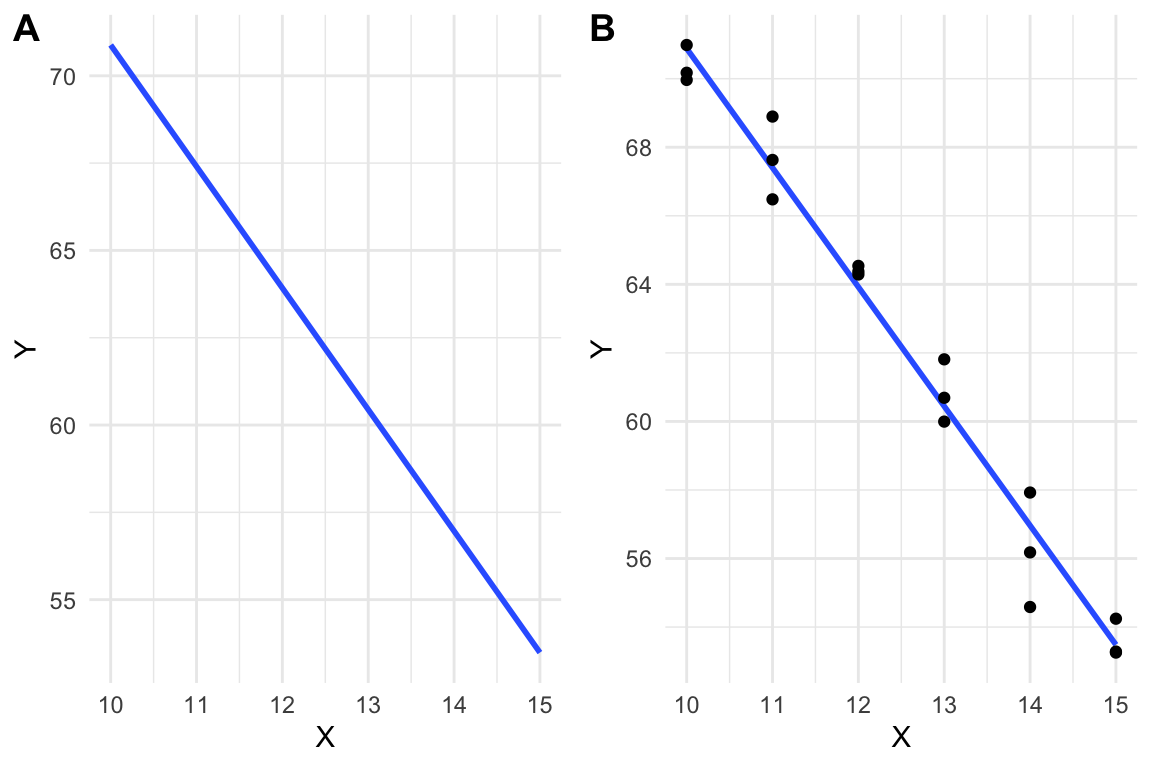
\includegraphics{Walker-elementary-statistical-modeling-draft_files/figure-latex/line-1.pdf}
\caption{\label{fig:line}A line vs.~a linear model. (A) the line \$y=-3.48X
+ 105.7 is drawn. (B) A linear model fit to the data. The model
coefficients are numerically equal to the slope and intercept of the
line in A.}
\end{figure}

All students are familiar with the idea of a linear model from learning
the equation of a line, which is

\begin{equation}
Y = mX + b
\label{eq:line}
\end{equation}

where \(m\) is the slope of the line and \(b\) is the \(Y\)-intercept.
It is useful to think of equation \eqref{eq:line} as a function that maps
values of \(X\) to values of \(Y\). Using this function, if we input
some value of \(X\), we always get the same value of Y as the output.

A linear model is a function, like that in equation \eqref{eq:line}, that
is fit to a set of data, often to model a process that generated the
data or something like the data. The line in Figure \ref{fig:line}A is
just that, a line, but the line in Figure \ref{fig:line}B is a model of
the data in Figure \ref{fig:line}B. The basic structure of a linear
model is

\begin{equation}
Y = \beta_0 + \beta_1 X + \varepsilon
\label{eq:lm}
\end{equation}

A linear model has two parts: the ``prediction''
(\(Y = \beta_0 + \beta_1 X\)) and the ``error'' (\(\varepsilon\)). The
prediction part looks like the equation for a line except that I've used
\(\beta_0\) for the intercept and \(\beta_1\) for the slope and I've put
the intercept term first. This re-labeling and re-arrangement make the
notation for a linear model more flexible for more complicated linear
models. For example
\(Y = \beta_0 + \beta_1 X_1 + \beta_2 X_2 + \varepsilon\) is a model
where \(Y\) is a function of two \(X\) variables.

As with the equation for a line, the prediction part of a linear model
is a function that maps a value of \(X\) to a specific value of \(Y\).
This mapped value is the \textbf{expected value} given a specific input
value of \(X\). This is often written as \(\mathrm{E}[Y|X]\). The error
part of a linear model is a random variable that adds some random value
to this expected value. Nothing about the model part of a linear model
can predict its value.

The inputs to a linear model (the \(X\) variables) have many names
including ``independent variables,'' ``predictor variables,'',
``explanatory variables,'' ``treatment variables,'' and ``covariates''.
The output of a linear model (the \(Y\) variable or variables if the
model is multivariate) is the ``dependent variable,'' ``response,'' or
``outcome.'' The \(\beta\) in the linear model are model
\textbf{parameters} There can be additional parameters in more
sophisticated models. The coefficients of the \(X\) in a linear model
(\(\beta_1\) in model \eqref{eq:lm}) are often called ``the effects'' (so
\(\beta_1\) is the effect of \(X_1\)).

Although a linear model is a model of a data-generating process, linear
models are not typically used to actually generate any data. Instead,
when we use a linear model to understand something about a real dataset,
we think of our data as one realization of a process that generates data
like ours. A linear model is a model of that process. That said, it is
incredibly useful to use linear models to create fake datasets for at
least two reasons: to probe our understanding of statistical modeling
generally and, more specifically, to check that a model actually creates
data like that in the real dataset that we are analyzing.

\subsection{Linear models are used for prediction, explanation, and
description}\label{linear-models-are-used-for-prediction-explanation-and-description}

Researchers typically use linear models to understand relationships
between one or more \(Y\) variables and one or more \(X\) variables.
These relationships include

\begin{enumerate}
\def\labelenumi{\arabic{enumi}.}
\item
  Descriptive modeling. Sometimes a researcher merely wants to describe
  the relationship between \(Y\) and a set of \(X\) variables, perhaps
  to discover patterns. For example, the arrival of a spring migrant
  bird (\(Y\)) as a function of sex (\(X_1\)) and age (\(X_2\)) might
  show that males and younger individuals arrive earlier. Importantly,
  if another \(X\) variable is added to the model (or one dropped), the
  coefficients, and therefore, the precise description, will change.
  That is, the interpretation of a coefficient as a descriptor is
  \emph{conditional} on the other covariates (\(X\) variables) in the
  model. In a descriptive model, there is no implication of causal
  effects and the goal is not prediction. Nevertheless, it is very hard
  for humans to discuss a descriptive model without using causal
  language, which probably means that it is hard for us to think of
  these models as \emph{mere description}. Like natural history,
  descriptive models are useful as patterns in want of an explanation,
  using more explicit causal models including experiments.
\item
  Predictive modeling. Predictive modeling is very common in applied
  research. For example, fisheries researchers might model the
  relationship between population density and habitat variables to
  predict which subset of ponds in a region are most suitable for brook
  trout (\emph{Salvelinus fontinalis}) reintroduction. The goal is to
  build a model with minimal prediction error, which is the error
  between predicted and actual values for a future sample. In predictive
  modeling, the \(X\) (``predictor'') variables are largely instrumental
  -- how these are related to \(Y\) is not a goal of the modeling,
  although sometimes an investigator may be interested in the relative
  importance among the \(X\) for predicting \(Y\) (for example,
  collecting the data may be time consuming, or expensive, or
  enviromentally destructive, so know which subset of \(X\) are most
  important for predicting \(Y\) is a useful strategy).
\item
  Explanatory (causal) modeling. Very often, researchers are explicitly
  interested in \emph{how} the \(X\) variables are causally related to
  \(Y\). The fisheries researchers that want to reintroduce trout may
  want to develop and manage a set of ponds to maintain healthy trout
  populations. This active management requires intervention to change
  habitat traits in a direction, and with a magnitude, to cause the
  desired response. This model is predictive -- a specific change in
  \(X\) predicts a specific response in \(Y\) -- because the
  coefficients of the model provide knowledge on how the system
  functions -- how changes in the inputs \emph{cause} change in the
  output. Causal interpretation of model coefficients requires a set of
  strong assumptions about the \(X\) variables in the model. These
  assumptions are typically met in \textbf{experimental designs} but not
  \textbf{observational designs}.
\end{enumerate}

With observational designs, biologists are often not very explicit about
which of these is the goal of the modeling and use a combination of
descriptive, predictive, and causal language to describe and discuss
results. Many papers read as if the researchers intend explanatory
inference but because of norms within the biology community, mask this
intention with ``predictive'' language. Here, I advocate embracing
explicit, explanatory modeling by being very transparent about the
model's goal and assumptions.

\section{Model fitting}\label{model-fitting}

In order to use a linear model to describe, predict, or explain, we need
to fit a model to data in order to estimate the parameters. If we fit
model \eqref{eq:fitlm} to some data, the estimated parameters are the
coefficients (\(b_0\) and \(b_1\)) of the fit model

\begin{equation}
\mathrm{E}[Y|X] = b_0 + b_1 X
\label{eq:fitlm}
\end{equation}

The left-hand side of equation \eqref{eq:fitlm} is the \textbf{conditional
expectation} and is read as ``the expectation of Y given X'' or ``the
expected value of Y given X''. Throughout this book, I use the greek
\(\beta\) to refer to a theoretical, data-generating parameter and the
roman ``b'' to refer its estimate.

The goal of descriptive and explanatory modeling is the estimate of the
coefficients of the \(X\) variables and their uncertainty. The goal of
predictive modeling is the estimate of predicted values, and their
uncertainty, given specific values of \(X\). These predicted values are
the conditional expectations.

\begin{figure}
\centering
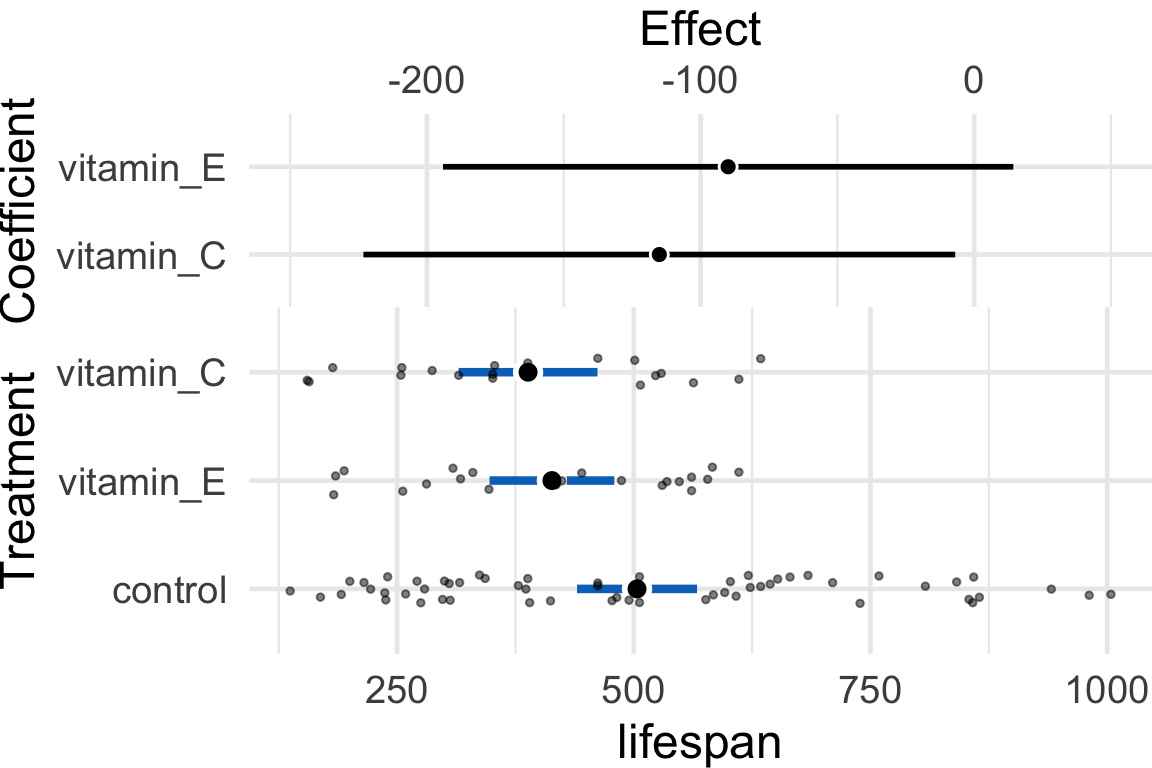
\includegraphics{Walker-elementary-statistical-modeling-draft_files/figure-latex/coldVoles-1.pdf}
\caption{\label{fig:coldVoles}HarrellPlot of vole data.}
\end{figure}

For the model fit to the data in Figure \ref{fig:line}B, the coefficient
of \(X\) is the slope of the line. Perhaps surprisingly, we can fit a
model like equation \eqref{eq:lm} to data in which the \(X\) variable is
categorical. A simple example is the experiment of antioxidants
(vitamins C and E) on lifespan in Voles (Fig. \ref{fig:coldVoles}). In
this experiment, the \(X\) variable is categorical, with three
\textbf{levels}: ``Control'', ``Vitamin\_E'' and ``Vitamin\_C''.
Categorical \(X\) variables are often called \textbf{factors}. The trick
to using a linear model with categorical \(X\) is to recode the factor
levels into numbers -- how this is done is explained in Chapter xxx.
When the \(X\) variable is categorical, the coefficients of the \(X\)
are \emph{differences in group means}. The linear model fit to the vole
data has two coefficients, one for Vitamin E and one for vitamin C. The
estimate and uncertainty of the these two coefficients are shown in the
top part of Figure \ref{fig:coldVoles}. The bottom part shows the raw
data, as well as the group (factor level) means and the uncertainty in
the estimate of these means.

The simplest possible model that can be fit to the data is

\begin{equation}
\mathrm{E}[Y] = b_0
\label{eq:unconditional}
\end{equation}

which is simply the mean of \(Y\), or, more specifically, the
\textbf{unconditional mean} of \(Y\), since its value is not conditional
on any value of \(X\).

\subsection{\texorpdfstring{``Statistical model'' not ``regression
model''}{Statistical model not regression model}}\label{statistical-model-not-regression-model}

Statistical modeling terminology can be confusing. The \(X\) variables
in a statistical model may be quantitative (continuous or integers) or
categorical (names or qualitative amounts) or some mix of the two.
Linear models with all quantitative independent variables are often
called ``regression models.'' Linear models with all categorical
independent variables are often called ``ANOVA models.'' Linear models
with a mix of quantitative and categorical variables are often called
``ANCOVA models'' if the focus is on one of the categorical \(X\) or
``regression models'' if there tend to be many independent variables.
Other patterns occur. For example ``ANCOVA models'' often include
interaction effects but ``regression models'' rarely do. To avoid
thinking of statistical analysis as ``regression vs.~ANOVA'', I will
most often use the term ``statistical model'' for general usage, and use
a more specific term only to emphasize something about the model in that
particluar context.

\section{Multilevel models}\label{multilevel-models}

\section{Linear models versus non-linear
models}\label{linear-models-versus-non-linear-models}

In this text, I use ``linear model'' for any model that is linear in the
parameters, which means that the different components of the model are
added together. Or, using the language of matrix algebra, the predictor
is a simple dot product of the model matrix and the coefficients. For
example, a cubic polynomial model

\begin{equation}
Y = \beta_0 + \beta_1 X + \beta_2 X^2 + \beta_3 X^3 + \varepsilon
\end{equation}

is a linear model, even though the function is non-linear, because the
different components are added (or, using matrix algebra, the predictor
is \(\mathbf{X}\boldsymbol{\beta}\)).

A generalized linear model (GLM) has the form \(g(\mu_i) = \eta_i\)
where \(\eta\) (the greek letter eta) is the linear predictor, which is
linear in the parameters.

\begin{equation}
\eta = \mathbf{X}\boldsymbol{\beta} 
\end{equation}

Many sources do not consider a GLM to be a ``linear model'' but an
``extension'' of a linear model. Regardless, a GLM is linear in the
parameters and here, I include GLMs under the ``linear model'' umbrella.

Non-linear models, in conrast to a GLM or classical linear model, are
not linear in the parameters (the predictor is not a simple dot product
of the model matrix and a vector of parameters). For example, the
Michaelis-Menten model is a nonlinear model

\begin{equation}
Y = \frac{\beta_1 X}{\beta_2 + X} + \varepsilon
\end{equation}

\chapter*{Appendix 1: Organization -- R Projects and R
Notebooks}\label{appendix-1-organization-r-projects-and-r-notebooks}
\addcontentsline{toc}{chapter}{Appendix 1: Organization -- R Projects
and R Notebooks}

\section{Importing Packages}\label{importing-packages}

The R scripts you write will include functions in packages that are not
included in Base R. These packages need to be downloaded from an
internet server to your computer. You only need to do this once. But,
each time you start a new R session, you will need to load a package
using the \texttt{library()} function. Now is a good time to import
packages that we will use

\begin{enumerate}
\def\labelenumi{\arabic{enumi}.}
\tightlist
\item
  Open R Studio and choose the menu item ``Tools'' \textgreater{}
  ``Install Packages''
\item
  In the ``packages'' input box, insert ``ggplot2, data.table, emmeans,
  lme4, reshape2''. Make sure that ``install dependencies'' is clicked
  before you click ``Install''
\end{enumerate}

Again, once these are installed, you don't need to do this again. You
simply need to use the \texttt{library()} function at the start of a
script.

\section{Create an R Studio Project for this
Class}\label{create-an-r-studio-project-for-this-class}

\begin{enumerate}
\def\labelenumi{\arabic{enumi}.}
\tightlist
\item
  Create a folder named ``BIO\_413''
\item
  Within this folder, create new folders named

  \begin{enumerate}
  \def\labelenumii{\arabic{enumii}.}
  \tightlist
  \item
    ``notebooks'' -- this is where your R notebooks are stored
  \item
    ``R'' -- this is where R scripts are stored
  \item
    ``data'' -- this is where data that we download from public archives
    are stored
  \item
    ``output'' -- this is where you will store fake data generated in
    this class
  \item
    ``images'' -- this is where image files are stored
  \end{enumerate}
\item
  Open R Studio and click the menu item File \textgreater{} New
  Project\ldots{}
\item
  Choose ``Existing Directory'' and navigate to your BIO\_413 folder
\item
  Choose ``Create Project''
\item
  Check that a file named ``BIO\_413.Rproj'' is in your BIO\_413 folder
\end{enumerate}

\section{R Notebooks}\label{r-notebooks}

A typical statistical modeling project will consist of:

\begin{enumerate}
\def\labelenumi{\arabic{enumi}.}
\tightlist
\item
  reading data from Excel or text (.csv or .txt) files
\item
  cleaning data
\item
  analysis
\item
  generating plots
\item
  generating tables
\item
  writing text to describe the project, the methods, the analysis, and
  the interpretation of the results (plots and tables)
\end{enumerate}

The best practice for reproducible research is to have all six of these
steps in your R Notebook. Too many research projects are not
reproducible because the data were cleaned in Excel, and then different
parts of the data were separately imported into a GUI statistics
software for analysis, and then output from the statistics software was
transcribed to Excel to make a table. And other parts of the analysis
are used to create a plot in some plotting software. And then the tables
and plots are pasted into Microsoft Word to create a report. Any change
at any step in this process will require the researcher to remember all
the downstream parts that are dependent on the change and to re-do an
analysis, or a table, or a plot, etc. etc.

The goal with an R Studio Notebook is to explicitly link all this so
that changes in earlier steps automatically flow into the later steps.
So, at the end of a project, a researcher can choose ``run all'' from
the menu and the data are read, cleaned, analyzed, ploted, tabled, and
put into a report with the text.

This means that you have to think of the organization of the R code that
your write in a Notebook. Your cannot simply append new code to the end
of a script if something earlier (or above) is dependent on it. You need
to go back up and insert the new code at some earlier (and meaningful)
point.

For example, an R chunk generates 100 random normal values and then
plots these with a histogram. This was the chunk that I wrote

\begin{Shaded}
\begin{Highlighting}[]
\NormalTok{x <-}\StringTok{ }\KeywordTok{rnorm}\NormalTok{(n)}
\KeywordTok{qplot}\NormalTok{(x)}
\end{Highlighting}
\end{Shaded}

When I ran the chunk, I got the error ``Error in rnorm(n) : object n not
found''. I was using the function \texttt{rnorm()} to generate values
but I hadn't assigned any value to \texttt{n} yet, so I got the error.
To get this to work properly, I could have just typed
\texttt{n\ \textless{}-\ 100} in the console and then re-run the script
but I want it to work properly on a fresh run of the chunk (after
quitting and re-opening R Studio) so I instead inserted
\texttt{n\ \textless{}-\ 100} at the start of the chunk, like this:

\begin{Shaded}
\begin{Highlighting}[]
\NormalTok{n <-}\StringTok{ }\DecValTok{100}
\NormalTok{x <-}\StringTok{ }\KeywordTok{rnorm}\NormalTok{(n)}
\KeywordTok{qplot}\NormalTok{(x)}
\end{Highlighting}
\end{Shaded}

\subsection{Create an R Notebook for this
Chapter}\label{create-an-r-notebook-for-this-chapter}

\begin{enumerate}
\def\labelenumi{\arabic{enumi}.}
\tightlist
\item
  The top-left icon in R Studio is a little plus sign within a green
  circle. Click this and choose ``R Notebook'' from the pull-down menu.
\item
  Change the title of the notebook to ``Notebook\_01-organization''
\item
  Delete the default R Markdown text starting with ``This is an {[}R
  Markdown{]}\ldots{}''
\end{enumerate}

Now write some text documenting which packages you installed.

\subsection{\texorpdfstring{Create a ``setup''
chunk}{Create a setup chunk}}\label{create-a-setup-chunk}

\begin{enumerate}
\def\labelenumi{\arabic{enumi}.}
\tightlist
\item
  Click on the ``Insert'' menu on the right hand side of the script (R
  Markdown) pane and choose ``R''. This will insert an R code chunk into
  your R markdown document.
\item
  The first R chunk of a notebook should be a setup chunk. Name the
  chunk ``setup''
\item
  load the libraries ggplot2 and data.table and click the chunk's run
  button (the green triangle to the right of the chunk)
\end{enumerate}

\begin{Shaded}
\begin{Highlighting}[]
\KeywordTok{library}\NormalTok{(ggplot2)}
\KeywordTok{library}\NormalTok{(data.table)}
\end{Highlighting}
\end{Shaded}

I added the chunk option ``message=FALSE''. Run your chunk with and
without this as an option.

\subsection{\texorpdfstring{Create a ``simple plot''
chunk}{Create a simple plot chunk}}\label{create-a-simple-plot-chunk}

\begin{enumerate}
\def\labelenumi{\arabic{enumi}.}
\setcounter{enumi}{3}
\tightlist
\item
  Create a new chunk and label it ``simple plot''
\item
  insert the following R script and then click the chunk's run button.
  Do you get a plot?
\end{enumerate}

\begin{Shaded}
\begin{Highlighting}[]
\NormalTok{n <-}\StringTok{ }\DecValTok{100}
\NormalTok{x <-}\StringTok{ }\KeywordTok{rnorm}\NormalTok{(n)}
\KeywordTok{qplot}\NormalTok{(x)}
\end{Highlighting}
\end{Shaded}

\begin{verbatim}
## `stat_bin()` using `bins = 30`. Pick better value with `binwidth`.
\end{verbatim}

\includegraphics{Walker-elementary-statistical-modeling-draft_files/figure-latex/simple plot-1.pdf}

\subsection{Create more R chunks and explore options and play with R
code}\label{create-more-r-chunks-and-explore-options-and-play-with-r-code}

\chapter*{Appendix 2: Data -- Reading, Writing, and
Fake}\label{appendix-2-data-reading-writing-and-fake}
\addcontentsline{toc}{chapter}{Appendix 2: Data -- Reading, Writing, and
Fake}

\section{Create new notebook for this
chapter}\label{create-new-notebook-for-this-chapter}

Be sure to save the notebook in the ``notebooks'' folder of your
BIO\_413 project. Annotate your notebook with notes! Update it as you
learn more! We will use data.table for importing text files in
tab-delimited or comma-separated formats and the readxl package for
importing excel files.

\begin{Shaded}
\begin{Highlighting}[]
\KeywordTok{library}\NormalTok{(ggplot2)}
\KeywordTok{library}\NormalTok{(ggpubr)}
\KeywordTok{library}\NormalTok{(data.table)}
\KeywordTok{library}\NormalTok{(readxl)}
\KeywordTok{library}\NormalTok{(emmeans)}
\KeywordTok{library}\NormalTok{(mvtnorm)}

\NormalTok{knitr}\OperatorTok{::}\NormalTok{opts_chunk}\OperatorTok{$}\KeywordTok{set}\NormalTok{(}\DataTypeTok{fig.width=}\DecValTok{6}\NormalTok{, }\DataTypeTok{fig.height=}\DecValTok{4}\NormalTok{) }
\end{Highlighting}
\end{Shaded}

\section{Importing Data}\label{importing-data}

Throughout this book, we will download data from the
\href{https://datadryad.org}{Dryad Digital Repository}, which is a major
resource for increasing reproducibility in science. My own view is that
\emph{all data} should be archived on some public server (exceptions
include data that are proprietary or contain sensitive information --
such as human health measures).

The downloaded data will be inserted into the ``data'' folder. To access
these data in an R script, the script needs to know ``where to look'' or
the ``address.'' This address is the \textbf{directory path}. The
default path for an R notebook is the directory containing the notebook
.Rmd file. This file should be in the ``notebooks'' folder within
``BIO\_413''. The ``BIO\_413'' Folder is the parent of the ``notebooks''
folder. It is also the parent of the ``data'' folder. To see any content
within the ``data'' folder, the R script needs to tell R to move back
(or up) the directory structure out of the ``notebooks'' folder into the
parent ``BIO\_413'' folder and then forward (or down) into the ``data''
folder. This is done with

\begin{Shaded}
\begin{Highlighting}[]
\NormalTok{data_path <-}\StringTok{ "../data"}
\end{Highlighting}
\end{Shaded}

The \texttt{..} moves the address (of where to read input or write
output) back one step and \texttt{/data} moves the address forward into
the ``data'' folder. This folder will eventually contains lots of data
from Dryad Digital Repository.

\subsection{Excel File}\label{excel-file}

The Excel dataset is from an experiment on the growth response of zebra
finch chicks to an incubation call that presumably signals ``hot
environment'' to the embryos
(\href{http://science.sciencemag.org/content/353/6301/812}{Mariette,
M.M. and Buchanan, K.L., 2016. Prenatal acoustic communication programs
offspring for high posthatching temperatures in a songbird. Science,
353(6301), pp.812-814}). The source file is from the Dryad Repository
here:

\textbf{file name}: ``allDatasetsMarietteBuchanan2016.xls''

\textbf{source}: \url{https://datadryad.org//handle/10255/dryad.122315}

Steps

\begin{enumerate}
\def\labelenumi{\arabic{enumi}.}
\tightlist
\item
  Copy the title of the Dryad page, which is ``Data from: Prenatal
  acoustic communication programs offspring for high post-hatching
  temperatures in a songbird''
\item
  Create a new folder within ``data'' and paste in the copied title as
  the folder name
\item
  Remove the colon from the name, so the folder name is ``Data from
  Prenatal acoustic communication programs offspring for high
  post-hatching temperatures in a songbird''
\item
  Download the .xls file into this folder
\end{enumerate}

A .xls file is an old (pre 2007) Microsoft Excel file type. It is a
binary file and can only be opened into a readable format with
specialized software. The more modern Excel file type is .xlsx, which
contains within it multiple xml components. An xml file is a text file,
and so contains readable content, but the content is xml code to display
something. In general, I am a big advocate of archiving stuff as text
files (manuscripts, data, scripts, blog posts) because these will
\emph{always} be readable by future software. Microsoft Excel is not
likely to die anytime soon and software that can read .xls and
especially .xlsx files (again, .xlsx files are text files) is even less
likely to disappear but we can feel even more confident if data are
archived as text files. That said, a single microsoft excel file with
multiple sheets is an efficient method for distributing data and the
readxl package provides excellent tools for reading different sheets of
a single .xls or .xlsx file.

The code below uses the function \texttt{read\_excel()} from the package
readxl. More about the amazing power of this package is the
\href{https://readxl.tidyverse.org}{tidyverse page} and
\href{http://r4ds.had.co.nz/data-import.html}{chapter 11} in the \emph{R
for Data Science} book.

\begin{Shaded}
\begin{Highlighting}[]
\NormalTok{data_folder <-}\StringTok{ "Data from Prenatal acoustic communication programs offspring for high post-hatching temperatures in a songbird"}
\NormalTok{filename <-}\StringTok{ "allDatasetsMarietteBuchanan2016.xls"}
\NormalTok{file_path <-}\StringTok{ }\KeywordTok{paste}\NormalTok{(data_path, data_folder, filename, }\DataTypeTok{sep=}\StringTok{"/"}\NormalTok{)}
\NormalTok{chick <-}\StringTok{ }\KeywordTok{data.table}\NormalTok{(}\KeywordTok{read_excel}\NormalTok{(file_path, }\DataTypeTok{sheet=}\StringTok{"nestlingMass"}\NormalTok{))}
\KeywordTok{head}\NormalTok{(chick) }\CommentTok{# check -- are there headers? are there the correct number of columns?}
\end{Highlighting}
\end{Shaded}

\begin{verbatim}
##       chick ID brood ID brood composition sex rank in nest
## 1:    N1.10LF3  N1.10m3             mixed   F            2
## 2: N1.10noCut3  N1.10m3             mixed   M            4
## 3:    N1.10RB3  N1.10m3             mixed   F            2
## 4:    N1.10RF3  N1.10m3             mixed   F            5
## 5:    N1.12LB3  N1.12m3             mixed   F            3
## 6:    N1.12LF3  N1.12m3             mixed   F            1
##    playback treatment nest temperature above ambient
## 1:              treat                       4.289583
## 2:               cont                       4.289583
## 3:               cont                       4.289583
## 4:               cont                       4.289583
## 5:               cont                       3.972917
## 6:              treat                       3.972917
##    max daily temp hatch day mean max temp hatch to day2
## 1:                     17.4                    18.83333
## 2:                     19.0                    20.53333
## 3:                     17.4                    18.83333
## 4:                     19.0                    20.53333
## 5:                     29.0                    24.63333
## 6:                     25.1                    24.80000
##    mean max temp hatch to day10 mean max temp hatch to day13 hatching mass
## 1:                        22.70                     23.05714           0.7
## 2:                        24.53                     23.41429           0.6
## 3:                        22.70                     23.05714           0.7
## 4:                        24.53                     23.41429           0.6
## 5:                        22.85                     22.91429           0.7
## 6:                        23.35                     23.24286           0.6
##    day1 mass day2 mass day10 mass day13 mass day13 tarsus
## 1:       1.1       1.2         NA        9.8        14.11
## 2:       0.8       1.1         NA        9.1        12.90
## 3:       0.9       1.4         NA        9.3        13.60
## 4:       0.5       0.9         NA        7.7        13.06
## 5:         1       1.4        9.4       10.1        14.08
## 6:       0.9       1.4        8.1        9.6        13.46
\end{verbatim}

\begin{center}\rule{0.5\linewidth}{\linethickness}\end{center}

\textbf{NOTE}

If you are getting errors when trying to read a file, it is probably a
bug in the construction of the variable \texttt{file\_path}, which is a
string variable and the value has to be exactly match the directly path
to the file you are trying to read. \texttt{file\_path} is constructed
by pasting together the variables \texttt{data\_path},
\texttt{data\_folder}, and \texttt{filename}. Type \texttt{file\_path}
into the console and look at the value. Then check

\begin{enumerate}
\def\labelenumi{\arabic{enumi}.}
\tightlist
\item
  Spelling. Humans are very good at understanding misspelled words but
  the R language (or any computer language) is very literal. ``../data''
  does not equal ``./data'' or ``../ data'' or ``../data''
\item
  Capitalization. R is \textbf{case sensitive} (some programming
  languages are not). ``../data'' does not equal ``../Data'' or
  ``../DATA''.
\item
  is the file you are trying to read actually in the folder you are
  trying to read from?
\item
  is the notebook that you are writing in the folder ``notebooks''? (the
  construction of \texttt{file\_path} assumes that notebook is one
  folder deep within the project folder.
\end{enumerate}

If the spelling or capitalization of any of these components is wrong,
then \texttt{file\_path} will be wrong. If there is any difference in
any character in the string, then R will return an error. So spelling
AND capitalization have to be perfect, not simply close. Humans are very
good at understanding misspelled and OdDLy capitalized words but the R
language (or any computer language) is very literal.

\begin{center}\rule{0.5\linewidth}{\linethickness}\end{center}

In this book, we will consistently uses the protocol for storing and
retrieving downloaded files. The first three lines in the script above
creates the directory path to the file. This path includes

\begin{enumerate}
\def\labelenumi{\arabic{enumi}.}
\tightlist
\item
  data\_path -- the relative path into the folder ``data'' (relative to
  the location of the notebook file)
\item
  data\_folder -- the name of the folder within ``data'' containing the
  file
\item
  filename -- the name of the file to read
\end{enumerate}

These are all put together into a single path using the function
\texttt{paste()}. Read about paste. It will be used repeatedly. The
\texttt{read\_excel(file\_path,\ sheet="nestlingMass")} reads the
nestlingMass sheet only. This function is embedded within the
\texttt{data.table()} function and so is converted into a data.table.
The data.table is assigned to the object ``chick''

The \texttt{head(chick)} script simply displays the first few lines of
the data.table. This is one way to check that the data were imported
correctly. In this case, it is easy to see that the column names have
spaces in them. It can sometimes be hard to work with column names with
spaces and so this next line of code changes all spaces to an underscore

\begin{Shaded}
\begin{Highlighting}[]
\KeywordTok{setnames}\NormalTok{(chick, }\DataTypeTok{old=}\KeywordTok{colnames}\NormalTok{(chick), }\DataTypeTok{new=}\KeywordTok{gsub}\NormalTok{(}\StringTok{" "}\NormalTok{, }\StringTok{"_"}\NormalTok{, }\KeywordTok{colnames}\NormalTok{(chick)))}
\end{Highlighting}
\end{Shaded}

Resist the temptation to change the column names in the data file, which
reduces reproducibility. Always increase reproducibility!

Just for fun, let's plot the data and reproduce Fig. 2A and B. We are
using the \texttt{qplot} function, which is from the ggplot2 package.
Two plots are made and only a subset of the rows are plotted in each (in
A, the subset in which playback\_treatment==``treat'' and, in B, the
subset in which playback\_treatment==``cont''). This book uses the
ggplot2 package extensively.

\begin{Shaded}
\begin{Highlighting}[]
\KeywordTok{qplot}\NormalTok{(}\DataTypeTok{x=}\NormalTok{nest_temperature_above_ambient, }\DataTypeTok{y=}\NormalTok{day13_mass, }\DataTypeTok{data=}\NormalTok{chick[playback_treatment}\OperatorTok{==}\StringTok{"treat"}\NormalTok{]) }\OperatorTok{+}
\StringTok{  }\KeywordTok{geom_smooth}\NormalTok{(}\DataTypeTok{method=}\StringTok{"lm"}\NormalTok{)}
\end{Highlighting}
\end{Shaded}

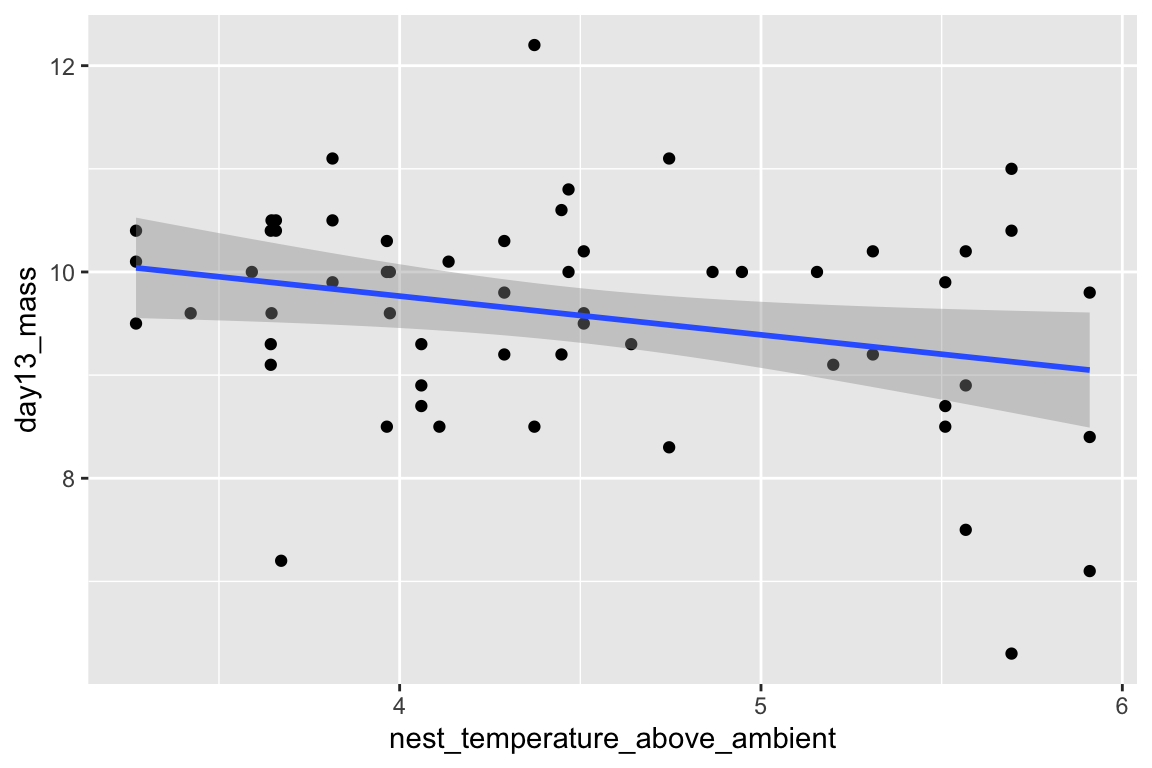
\includegraphics{Walker-elementary-statistical-modeling-draft_files/figure-latex/plotchickdata-1.pdf}

\begin{Shaded}
\begin{Highlighting}[]
\KeywordTok{qplot}\NormalTok{(}\DataTypeTok{x=}\NormalTok{nest_temperature_above_ambient, }\DataTypeTok{y=}\NormalTok{day13_mass, }\DataTypeTok{data=}\NormalTok{chick[playback_treatment}\OperatorTok{==}\StringTok{"cont"}\NormalTok{]) }\OperatorTok{+}
\StringTok{  }\KeywordTok{geom_smooth}\NormalTok{(}\DataTypeTok{method=}\StringTok{"lm"}\NormalTok{)}
\end{Highlighting}
\end{Shaded}

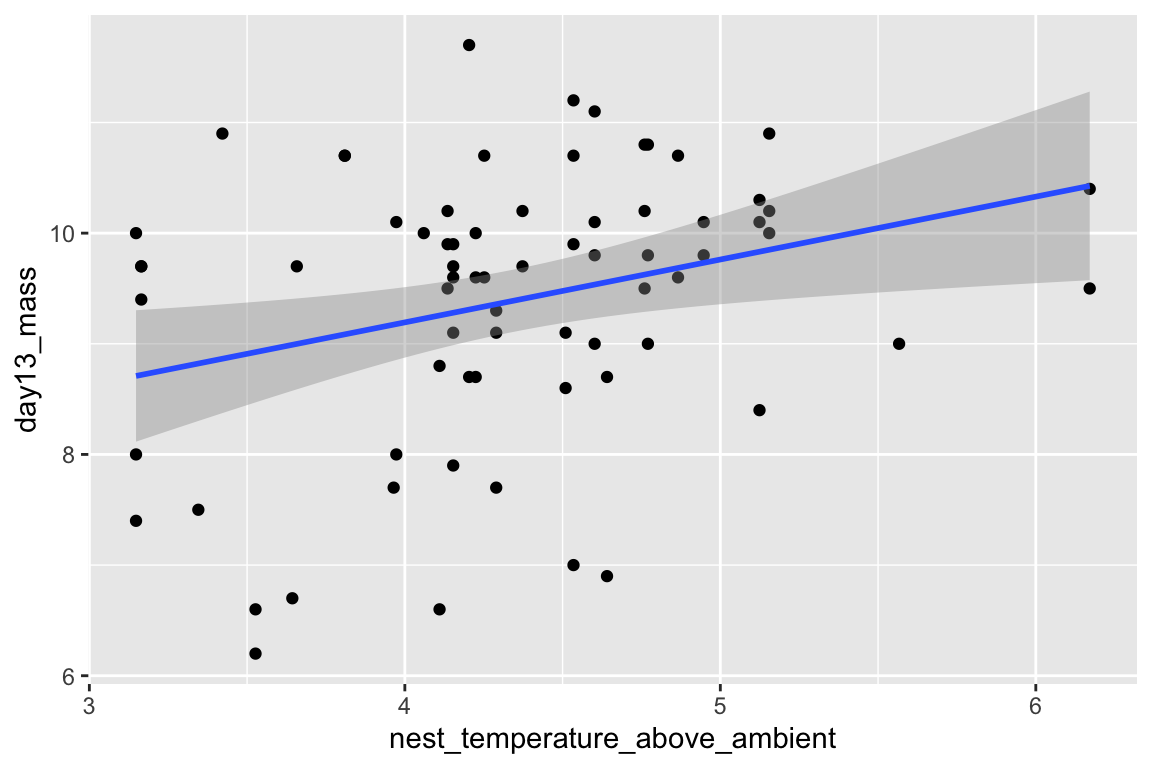
\includegraphics{Walker-elementary-statistical-modeling-draft_files/figure-latex/plotchickdata-2.pdf}

\subsection{Text File}\label{text-file}

The example dataset comes from an experiment on the effect of
\href{http://science.sciencemag.org/content/early/2012/03/28/science.1215025}{neonicotinoid
pesticides on bumble bee colony growth}.

\textbf{file name}: ``Whitehorn, O'Connor, Wackers, Goulson (2012) Data
from `Neonicotinoid pesticide reduces bumblebee colony growth and queen
production'.csv.csv''

\textbf{source}:
\url{https://datadryad.org//resource/doi:10.5061/dryad.1805c973}

Steps

\begin{enumerate}
\def\labelenumi{\arabic{enumi}.}
\tightlist
\item
  Copy the title of the Dryad page, which is ``Data from: Neonicotinoid
  pesticide reduces bumblebee colony growth and queen production''
\item
  Create a new folder within ``data'' and paste in the copied title as
  the folder name
\item
  Remove the colon from the name, so the folder name is ``Data from
  Neonicotinoid pesticide reduces bumblebee colony growth and queen
  production''
\item
  Download the .csv file into this folder
\end{enumerate}

A .csv file is a text file that is comma-delimted, which means that the
entries of a row are separated by commas. A text file is readable by any
text editor software and most other kinds of software. Datasets that are
stored as text files are typically saved as either .csv (where the
entries of a row are separated by commas) or .txt (where the entries are
separated by tabs). The base R way to read a .csv file is using
\texttt{read.csv}. The \texttt{read.table} function is more versatile,
as the delimiter can be specified. The function \texttt{fread()} from
the data.table package is fast, smart, and flexible. It is smart in the
sense that it guesses what the delimter is. Unfortunately, because of
spaces in the column labels for this file, fread guesses incorrectly
(another reason why spaces in column labels should be avoided). To
overcome this, the statement below specifies that the file contains a
``header'' (a line containing column labels)

\begin{Shaded}
\begin{Highlighting}[]
\NormalTok{data_folder <-}\StringTok{ "Data from Neonicotinoid pesticide reduces bumblebee colony growth and queen production"}
\NormalTok{filename <-}\StringTok{ "Whitehorn, O'Connor, Wackers, Goulson (2012) Data from 'Neonicotinoid pesticide reduces bumblebee colony growth and queen production'.csv.csv"}
\NormalTok{file_path <-}\StringTok{ }\KeywordTok{paste}\NormalTok{(data_path, data_folder, filename, }\DataTypeTok{sep=}\StringTok{"/"}\NormalTok{)}
\NormalTok{bee <-}\StringTok{ }\KeywordTok{fread}\NormalTok{(file_path, }\DataTypeTok{header=}\OtherTok{TRUE}\NormalTok{)}
\NormalTok{bee[, Treatment}\OperatorTok{:}\ErrorTok{=}\KeywordTok{factor}\NormalTok{(Treatment, }\KeywordTok{c}\NormalTok{(}\StringTok{"Control"}\NormalTok{, }\StringTok{"Low"}\NormalTok{, }\StringTok{"High"}\NormalTok{))]}
\KeywordTok{head}\NormalTok{(bee)}
\end{Highlighting}
\end{Shaded}

\begin{verbatim}
##    Treatment Nest ID No. workers      0      1      2   3   4    5    6
## 1:   Control      C1          13 712.95 748.30 800.57 865 966  997  850
## 2:   Control      C2          14 719.58 750.00 789.25 822 812  846  827
## 3:   Control      C3          17 704.92 736.31 767.99 837 976 1117 1050
## 4:   Control      C4          20 726.42 763.31 795.60 813 801  784   NA
## 5:   Control      C5          28 740.60 785.52 808.42 837 871  906  886
## 6:   Control      C6          15 727.10 751.90 774.80 807 847  859  827
##      7   8 V13 Workers left Males New queens Total unhatched pupae
## 1: 791 775  NA            2     0          1                    NA
## 2: 820 802  NA            6    15          0                    20
## 3: 866 808  NA            1     0          9                    NA
## 4:  NA  NA  NA            0     0          0                    12
## 5: 807 775  NA            3     0          0                    NA
## 6:  NA  NA  NA            0     0          0                   118
##    Queen pupae Empty cells
## 1:          NA          NA
## 2:           0         120
## 3:          NA          NA
## 4:           0          72
## 5:          NA          NA
## 6:          20         132
\end{verbatim}

Here, as with the import of the Excel file, the first three lines create
the directory path to the file. The treatment column is a factor
variable containing three levels (Control, Low, and High). R
automatically orders these alphabetically. For plotting and analysis, we
might want a different order. For example, we want Control to be first
in the order, since this is a natural ``reference'' level (what
everything is compared to). And if we think of ``Control'' as no
treatment, then it makes sense to have ``Low'' second in order and
``Hight'' last in order. The line
\texttt{bee{[},\ Treatment:=factor(Treatment,\ c("Control",\ "Low",\ "High")){]}}
re-orders these levels to this more meaningful order.

Again, there are spaces in the column names. \textbf{Here I'll leave it
to you to change this}

Here is a reproduction of Fig 2.

\begin{Shaded}
\begin{Highlighting}[]
\KeywordTok{ggbarplot}\NormalTok{(}\DataTypeTok{data=}\NormalTok{bee, }\DataTypeTok{x=}\StringTok{"Treatment"}\NormalTok{, }\DataTypeTok{y=}\StringTok{"New_queens"}\NormalTok{, }\DataTypeTok{add =} \KeywordTok{c}\NormalTok{(}\StringTok{"mean_se"}\NormalTok{))}
\end{Highlighting}
\end{Shaded}

\includegraphics{Walker-elementary-statistical-modeling-draft_files/figure-latex/plot bee fig. 2-1.pdf}

The plot suggests immediately some problems with the plot itself and the
associated analysis. First, the y-axis is counts, which means that
negative values are impossible. But the standard error bars look like
they use standard errors computed from a model that allows infinetly
large negative values, and the illustrated standard error bars imply
that negative values exist. So these error bars are misleading. Second,
it is good practice, especially if sample sizes are modest or small, to
``show the data'', which means, show the individual data points and not
just a summary of the distribution.

Here are three alternative plots for exploratory purposes. The first
simply ``shows the data'' but still uses the misleading standard error
bars. The second uses a box plot. The last plots the means and 95\%
confidence intervals modeled with a GLM (generalized linear model) to
account for the count data (the model used could be improved). Notice
that the bar length above the mean is longer than the bar length below
the mean (that is the interval is asymmetric about the mean). In order
to stay focussed on importing data, I leave explanation of these plots
and analysis to later chapters.

\begin{Shaded}
\begin{Highlighting}[]
\KeywordTok{ggbarplot}\NormalTok{(}\DataTypeTok{data=}\NormalTok{bee, }\DataTypeTok{x=}\StringTok{"Treatment"}\NormalTok{, }\DataTypeTok{y=}\StringTok{"New_queens"}\NormalTok{, }\DataTypeTok{add =} \KeywordTok{c}\NormalTok{(}\StringTok{"mean_se"}\NormalTok{, }\StringTok{"point"}\NormalTok{))}
\end{Highlighting}
\end{Shaded}

\includegraphics{Walker-elementary-statistical-modeling-draft_files/figure-latex/alternative plots-1.pdf}

\begin{Shaded}
\begin{Highlighting}[]
\KeywordTok{ggboxplot}\NormalTok{(}\DataTypeTok{data=}\NormalTok{bee, }\DataTypeTok{x=}\StringTok{"Treatment"}\NormalTok{, }\DataTypeTok{y=}\StringTok{"New_queens"}\NormalTok{)}
\end{Highlighting}
\end{Shaded}

\includegraphics{Walker-elementary-statistical-modeling-draft_files/figure-latex/alternative plots-2.pdf}

\begin{Shaded}
\begin{Highlighting}[]
\NormalTok{fit.glm <-}\StringTok{ }\KeywordTok{glm}\NormalTok{(New_queens }\OperatorTok{~}\StringTok{ }\NormalTok{Treatment, }\DataTypeTok{data=}\NormalTok{bee, }\DataTypeTok{family=}\KeywordTok{poisson}\NormalTok{())}
\NormalTok{means.glm <-}\StringTok{ }\KeywordTok{emmeans}\NormalTok{(fit.glm, }\DataTypeTok{specs=}\StringTok{"Treatment"}\NormalTok{, }\DataTypeTok{type =} \StringTok{"response"}\NormalTok{)}
\NormalTok{gg <-}\StringTok{ }\KeywordTok{ggplot}\NormalTok{(}\DataTypeTok{data=}\KeywordTok{data.frame}\NormalTok{(means.glm), }\KeywordTok{aes}\NormalTok{(}\DataTypeTok{x=}\NormalTok{Treatment, }\DataTypeTok{y=}\NormalTok{rate)) }\OperatorTok{+}
\StringTok{  }\KeywordTok{geom_col}\NormalTok{(}\DataTypeTok{fill=}\StringTok{"gray"}\NormalTok{) }\OperatorTok{+}\StringTok{ }
\StringTok{  }\KeywordTok{geom_errorbar}\NormalTok{(}\KeywordTok{aes}\NormalTok{(}\DataTypeTok{x=}\NormalTok{Treatment, }\DataTypeTok{ymin=}\NormalTok{asymp.LCL, }\DataTypeTok{ymax=}\NormalTok{asymp.UCL), }\DataTypeTok{width=}\FloatTok{0.3}\NormalTok{) }\OperatorTok{+}
\StringTok{  }\KeywordTok{ylab}\NormalTok{(}\StringTok{"New queens"}\NormalTok{) }\OperatorTok{+}
\StringTok{  }\OtherTok{NULL}
\NormalTok{gg}
\end{Highlighting}
\end{Shaded}

\includegraphics{Walker-elementary-statistical-modeling-draft_files/figure-latex/alternative plots-3.pdf}

\section{Creating Fake Data}\label{creating-fake-data}

\subsection{Continuous X (fake observational
data)}\label{continuous-x-fake-observational-data}

A very simple simulation of a regression model

\begin{Shaded}
\begin{Highlighting}[]
\NormalTok{n <-}\StringTok{ }\DecValTok{25}
\NormalTok{beta_}\DecValTok{0}\NormalTok{ <-}\StringTok{ }\DecValTok{25}
\NormalTok{beta_}\DecValTok{1}\NormalTok{ <-}\StringTok{ }\FloatTok{3.4}
\NormalTok{sigma <-}\StringTok{ }\DecValTok{2}
\NormalTok{x <-}\StringTok{ }\KeywordTok{rnorm}\NormalTok{(n)}
\NormalTok{y <-}\StringTok{ }\NormalTok{beta_}\DecValTok{0} \OperatorTok{+}\StringTok{ }\NormalTok{beta_}\DecValTok{1}\OperatorTok{*}\NormalTok{x }\OperatorTok{+}\StringTok{ }\KeywordTok{rnorm}\NormalTok{(n, }\DataTypeTok{sd=}\NormalTok{sigma)}
\KeywordTok{qplot}\NormalTok{(x, y)}
\end{Highlighting}
\end{Shaded}

\includegraphics{Walker-elementary-statistical-modeling-draft_files/figure-latex/continuous X-1.pdf}

\begin{Shaded}
\begin{Highlighting}[]
\NormalTok{knitr}\OperatorTok{::}\KeywordTok{kable}\NormalTok{(}\KeywordTok{coefficients}\NormalTok{(}\KeywordTok{summary}\NormalTok{(}\KeywordTok{lm}\NormalTok{(y }\OperatorTok{~}\StringTok{ }\NormalTok{x))), }\DataTypeTok{digits=}\DecValTok{2}\NormalTok{)}
\end{Highlighting}
\end{Shaded}

\begin{tabular}{l|r|r|r|r}
\hline
  & Estimate & Std. Error & t value & Pr(>|t|)\\
\hline
(Intercept) & 24.46 & 0.39 & 62.43 & 0\\
\hline
x & 3.05 & 0.37 & 8.25 & 0\\
\hline
\end{tabular}

The coefficient of \(x\) is the ``Estimate''. How close is the estimate?
Run the simulation several times to look at the variation in the
estimate -- this will give you a sense of the uncertainty. Increase
\(n\) and explore this uncertainty. Increase all the way up to
\(n=10^5\). Commenting out the qplot line will make this exploration
easier.

\subsection{Categorical X (fake experimental
data)}\label{categorical-x-fake-experimental-data}

\begin{Shaded}
\begin{Highlighting}[]
\NormalTok{n <-}\StringTok{ }\DecValTok{5}

\NormalTok{fake_data <-}\StringTok{ }\KeywordTok{data.table}\NormalTok{(}\DataTypeTok{Treatment=}\KeywordTok{rep}\NormalTok{(}\KeywordTok{c}\NormalTok{(}\StringTok{"control"}\NormalTok{, }\StringTok{"treated"}\NormalTok{), }\DataTypeTok{each=}\NormalTok{n))}
\NormalTok{beta_}\DecValTok{0}\NormalTok{ <-}\StringTok{ }\FloatTok{10.5} \CommentTok{# mean of untreated}
\NormalTok{beta_}\DecValTok{1}\NormalTok{ <-}\StringTok{ }\FloatTok{2.1} \CommentTok{# difference in means (treated - untreated)}
\NormalTok{sigma <-}\StringTok{ }\DecValTok{3} \CommentTok{# the error standard deviation}
\CommentTok{# the Y variable ("Response") is a function of treatment. We use some matrix}
\CommentTok{# algebra to get this done.}
\CommentTok{# Turn the Treatment assignment into a model matrix. Take a peak at X!}
\NormalTok{X <-}\StringTok{ }\KeywordTok{model.matrix}\NormalTok{(}\OperatorTok{~}\StringTok{ }\NormalTok{Treatment, fake_data)}
\CommentTok{# to make the math easier the coefficients are collected into a vector}
\NormalTok{beta <-}\StringTok{ }\KeywordTok{c}\NormalTok{(beta_}\DecValTok{0}\NormalTok{, beta_}\DecValTok{1}\NormalTok{)}
\CommentTok{# you will see the formula Y=Xb many times. Here it is coded in R}
\NormalTok{fake_data[, Response}\OperatorTok{:}\ErrorTok{=}\NormalTok{X}\OperatorTok\NormalTok{beta }\OperatorTok{+}\StringTok{ }\KeywordTok{rnorm}\NormalTok{(n, }\DataTypeTok{sd=}\NormalTok{sigma)]}
\CommentTok{# plot it with a strip chart (often called a "dot plot")}
\KeywordTok{ggstripchart}\NormalTok{(}\DataTypeTok{data=}\NormalTok{fake_data, }\DataTypeTok{x=}\StringTok{"Treatment"}\NormalTok{, }\DataTypeTok{y=}\StringTok{"Response"}\NormalTok{, }\DataTypeTok{add =} \KeywordTok{c}\NormalTok{(}\StringTok{"mean_se"}\NormalTok{))}
\end{Highlighting}
\end{Shaded}

\includegraphics{Walker-elementary-statistical-modeling-draft_files/figure-latex/categorical X-1.pdf}

\begin{Shaded}
\begin{Highlighting}[]
\CommentTok{# fit using base R linear model function}
\NormalTok{fit <-}\StringTok{ }\KeywordTok{lm}\NormalTok{(Response }\OperatorTok{~}\StringTok{ }\NormalTok{Treatment, }\DataTypeTok{data=}\NormalTok{fake_data)}
\CommentTok{# display a pretty table of the coefficients}
\NormalTok{knitr}\OperatorTok{::}\KeywordTok{kable}\NormalTok{(}\KeywordTok{coefficients}\NormalTok{(}\KeywordTok{summary}\NormalTok{(fit)), }\DataTypeTok{digits=}\DecValTok{3}\NormalTok{)}
\end{Highlighting}
\end{Shaded}

\begin{tabular}{l|r|r|r|r}
\hline
  & Estimate & Std. Error & t value & Pr(>|t|)\\
\hline
(Intercept) & 11.528 & 1.521 & 7.579 & 0.000\\
\hline
Treatmenttreated & 2.100 & 2.151 & 0.976 & 0.358\\
\hline
\end{tabular}

Check that the intercept is close to beta\_0 and the coefficient for
Treatment is close to beta\_1. This coefficient is the different in
means between the treatment levels. It is the simulated effect. Again,
change \(n\). Good values are \(n=20\) and \(n=100\). Again, comment out
the plot line to make exploration more efficient.

\section{Saving Data}\label{saving-data}

Let's save the fake data to the ``Fake\_Data'' folder. In the ``output''
folder create a new folder named ``week 01''. Then set the path to the
output folder:

\begin{Shaded}
\begin{Highlighting}[]
\NormalTok{output_path <-}\StringTok{ "../output"} \CommentTok{# out to parent directory than down into Fake_data}
\end{Highlighting}
\end{Shaded}

This could be done at the beginning of the notebook, especially if many
output files are saved. Regardless, now complete the file\_path with the
specifics of this save.

\begin{Shaded}
\begin{Highlighting}[]
\NormalTok{data_folder <-}\StringTok{ "week 01"}
\NormalTok{filename <-}\StringTok{ "my_first_fake_data.txt"}
\NormalTok{file_path <-}\StringTok{ }\KeywordTok{paste}\NormalTok{(output_path, data_folder, filename, }\DataTypeTok{sep=}\StringTok{"/"}\NormalTok{)}
\KeywordTok{write.table}\NormalTok{(fake_data, file_path, }\DataTypeTok{sep=}\StringTok{"}\CharTok{\textbackslash{}t}\StringTok{"}\NormalTok{, }\DataTypeTok{quote=}\OtherTok{FALSE}\NormalTok{)}
\end{Highlighting}
\end{Shaded}

We used \texttt{write.table()} to create a tab-delimited text file using
\texttt{sep="\textbackslash{}t"} to specify tabs to separate the row
elements. ``\t'' is the standard character string for a tab. Check in
your Fake\_Data folder and open the file in a text editor.

\section{Problems}\label{problems}

\begin{enumerate}
\def\labelenumi{\arabic{enumi}.}
\item
  Download the dataset ``data-Lodjak.et.al-2016-FuncEcol.xlsx'' from the
  Dryad repository at
  \url{https://datadryad.org/resource/doi:10.5061/dryad.rd01s}. The
  .xlsx file presents the data cleanly but the trade-off is that the 1)
  multiple header rows, and 2) spaces in the header labels, 3)
  parentheses in the header labels make it more complex to import in a
  usable way. Import the data and plot Body Mass against Age (that is
  make Body Mass the ``Y'' variable and Age the ``X'' variable) using
  the qplot function. You should recode the column labels to remove
  spaces and parentheses using the setnames function.
\item
  Download the dataset ``Results2015.txt'' from the Dryad repository at
  \url{https://datadryad.org//resource/doi:10.5061/dryad.65vk4}. Try to
  reproduce Fig. 1. It's not easy. I've inserted the figure below.
\item
  (grad students only) Download and plot data from a Dryad Repository
  dataset of your choice.
\item
  (grad students only) Create fake experimental data with three
  treatment levels (control, lo\_temp, high\_temp). This will require
  three parameters: an intercept (beta\_0), an effect of lo\_temp
  (beta\_1), and an effect of high\_temp (beta\_2). You should be able
  to plug and play from the script above even if you don't underdstand
  at this point what any of it is! Plot it as a strip chart, as above.
\end{enumerate}

\begin{figure}
\centering
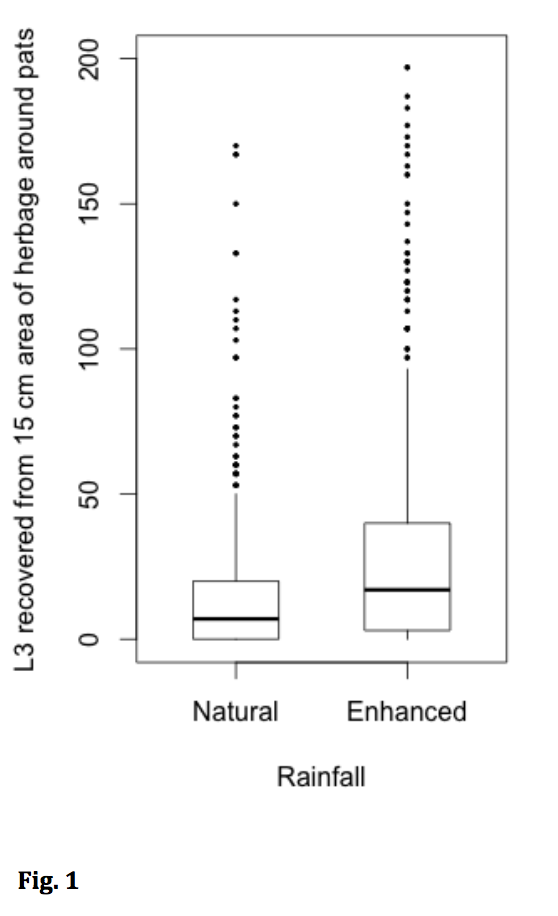
\includegraphics[width=0.50000\textwidth]{images/Dung_beetles_reduce_livestock-fig_1.png}
\caption{Fig. 1 from ``Dung beetles reduce livestock\ldots{}''}
\end{figure}

\chapter{Variability and Uncertainty (Standard Deviations and Standard
Errors)}\label{variability-and-uncertainty-standard-deviations-and-standard-errors}

\textbf{Uncertainty} is the stuff of science. A major goal of statistics
is measuring uncertainty. What do we mean by uncertainty? Uncertainty is
the error in estimating a parameter, such as the mean of a sample, or
the difference in means between two experimental treatments, or the
predicted response given a certain change in conditions. Uncertainty is
measured with a \textbf{variance} or its square root, which is a
\textbf{standard deviation}. The standard deviation of a statistic is
also (and more commonly) called a \textbf{standard error}.

Uncertainty emerges because of variability. In any introductory
statistics class, students are introduced to two measures of
variability, the ``standard deviation'' and the ``standard error.''
These terms are absolutely fundamental to statistics -- they are the
start of everything else. Yet, many biology professors confuse these
terms and certainly, introductory students do too.

When a research biologist uses the term ``standard deviation,'' they are
probably referring to the sample standard deviation which is a measure
of the variability of a sample. When a research biologist uses the term
``standard error,'' they are probably referring to the standard error of
a mean, but it could be the standard error of another statistics, such
as a regression slope. An important point to remember and understand is
that all standard errors \emph{are} standard deviations. This will make
more sense soon.

\section{The sample standard deviation vs.~the standard error of the
mean}\label{the-sample-standard-deviation-vs.the-standard-error-of-the-mean}

\subsection{Sample standard deviation}\label{sample-standard-deviation}

The sample standard deviation is a measure of the variability of a
sample. For example, were we to look at a histological section of
skeletal muscle we would see that the diameter of the fibers (the muscle
cells) is variable. We could use imaging software to measure the
diameter of a sample of 100 cells and get a \textbf{distribution} like
this

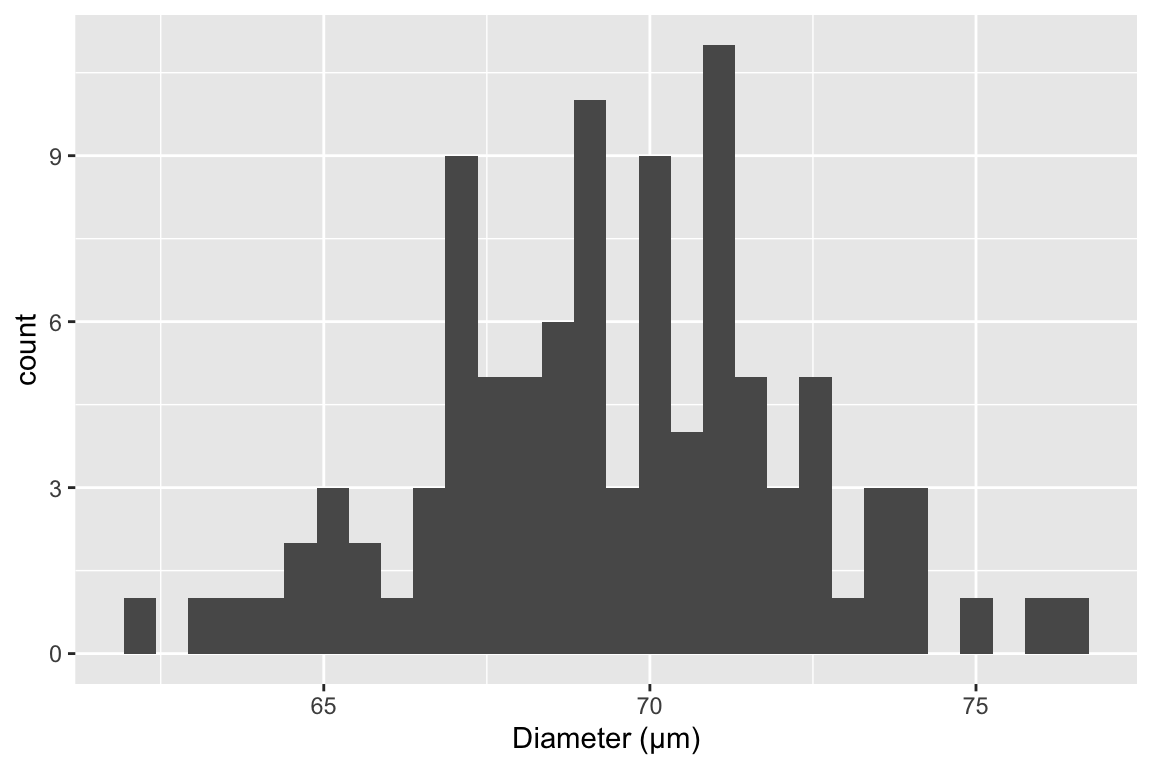
\includegraphics{Walker-elementary-statistical-modeling-draft_files/figure-latex/histogram-1.pdf}

The mean of this sample is 69.4 and the standard deviation is 2.8. The
standard deviation is the square root of the variance, and so computed
by

\begin{equation}
s_y = \sqrt{\frac{\sum_{i=1}^n{(y_i - \overline{y})^2}}{n-1}}
\label{eq:variance}
\end{equation}

Memorize this equation. To understand the logic of this measure of
variability, note that \(y_i - \overline{y}\) is the deviation of the
\(i\)th value from the sample mean, so the numerator is the sum of
squared deviations. The numerator is a sum over \(n\) items and the
denominator is \(n-1\) so the variance is (almost!) an averaged squared
deviation. More variable samples will have bigger deviations and,
therefore, bigger average squared deviations. Since the standard
deviation is the square root of the variance, a standard deviation is
the square root of the average squared deviation, it can be thought of
as a (not ``the'') measure of an average deviation.

Notes on the variance and standard deviation

\begin{enumerate}
\def\labelenumi{\arabic{enumi}.}
\tightlist
\item
  Variances are additive but standard deviations are not. This means
  that the variance of the sum of two independent (uncorrelated) random
  variables is simply the sum of the variances of each of the variables.
  This is important for many statistical analyses.
\item
  The units of variance are the square of the original units, which is
  awkward for interpretation. The units of a standard deviation is the
  same as that of the original variable, and so is much easier to
  interpet.
\item
  For variables that are approximately normally distributed, we can map
  the standard deviation to the quantiles of the distribution. For
  example, 68\% of the values are within one standard deviation of the
  mean, 95\% of the values are within two standard deviations, and 99\%
  of the values are within three standard deviations.
\end{enumerate}

\subsection{Standard error of the
mean}\label{standard-error-of-the-mean}

A standard error of a statistic is a measure of the precision of the
statistic. The standard error of the mean is a measure of the precision
of the mean. The smaller the value the more precise the estimate. The
standard error of the mean (SEM) is computed as

\begin{equation}
SEM = \frac{s_y}{\sqrt{n}}
\label{eq:se}
\end{equation}

The SEM is often denoted \(s_{\bar{y}}\) to indicate that it is a
standard deviation of the mean (\(\bar{y}\)). In what sense is a
standard error a measure of variability? This is kinda weird. If we
sample 100 cells cells in the slide one time and compute the mean
diameter, how can the mean have a standard deviation? There is only one
value! To understand how the SEM is a standard deviation, imagine
resampling 100 cells and recomputing a mean an infinite number of times
and each time, you write down the newly computed mean. The standard
error of the mean is the standard deviation of this infinitely long
column of means.

Notes on standard errors

\begin{enumerate}
\def\labelenumi{\arabic{enumi}.}
\tightlist
\item
  The SEM is only one kind of standard error. A standard deviation can
  be computed for any statistics -- these are all standard errors. For
  some statistics, such as the mean, the standard error can be computed
  directly using an equation, such as that for the SEM (equation
  @ref\{eq:se\}). For other statistics, a computer intensive method such
  as the \textbf{bootstrap} is necessary to compute a standard error. We
  will return to the bootstrap shortly.
\item
  The units of a standard error are the units of the measured variable.
\item
  A standard error is proportional to sample variability (the sample
  standard deviation, \(s_y\)) and inversely proportional to sample size
  (\(n\)). Sample variability is a function of both natural variation
  (there really is variation in diameter among fibers in the quadriceps
  muscle) and measurement error (imaging software with higher resolution
  can measure a diameter with less error). Since the SEM is a measure of
  the precision of estimating a mean, this means this precision will
  increase (or the SEM will decrease) if 1) an investigator uses methods
  that reduce measurement error and 2) an investigator computes the mean
  from a larger sample.
\item
  This last point (the SEM decreases with sample size) seems obvious
  when looking at equation @ref\{eq:se\}, since \(n\) is in the
  denominator. Of course \(n\) is also in the denominator of equation
  @ref\{eq:variance\} for the sample standard deviation (eq) but the
  standard deviation does not decrease as sample size increases. First
  this would make any sense -- variability is variability. A sample of
  10,000 cell diameters should be no more variable than a sample of 100
  cell diameters. Second, this should also be obvious from equation
  @ref\{eq:variance\}. The standard deviation is the square root of an
  average and averages don't increase with the number of things measured
  since both the the numerator (a sum) and denominator increase with
  \(n\).
\end{enumerate}

\section{Using Google Sheets to generate fake data to explore
uncertainty}\label{using-google-sheets-to-generate-fake-data-to-explore-uncertainty}

In statistics we are interested in estimated parameters of a
\textbf{population} using measures from a \textbf{sample}. The goal in
this section is to use Google Sheets (or Microsoft Excel) to use fake
data to discover the behavior of sampling and to gain some intuition
about uncertainty using standard errors.

\subsection{Steps}\label{steps}

\begin{enumerate}
\def\labelenumi{\arabic{enumi}.}
\tightlist
\item
  Open Google Sheets
\item
  In cell A1 type ``mu''. mu is the greek letter \(\mu\) and is very
  common notation for the poplation value (the TRUE value!) of the mean
  of some hypothetical measure. In cell B1, insert some number as the
  value of \(\mu\). Any number! It can be negative or positive.
\item
  In cell A2 type ``sigma''. sigma is the greek letter \(\sigma\).
  \(\sigma^2\) is very common (universal!) notation for the population
  (TRUE) variance of some measure or parameter. Notice that the true
  (population) values of the mean and variance are greek letters. This
  is pretty standard in statistics. In cell B2, insert some positive
  number (standard deviations are the positive square roots of the
  variance).
\item
  In cell A8 type the number 1
\item
  In cell A9 insert the equation ``=A8 + 1''. What is this equation
  doing? It is adding the number 1 to to the value in the cell above, so
  the resulting value should be 2.
\item
  In Cell B8, insert the equation ``=normsinv(rand())*\$B\$2 + \$B\$1``.
  The first part of the equation creates a random normal variable with
  mean 0 and standard deviation 1. multiplication and addition transform
  this to a random normal variable with mean \(\mu\) and standard
  deviation \(\sigma\) (the values you set in cells B1 and B2).
\item
  copy cell B8 and paste into cell B9. Now Higlight cells A9:B9 and copy
  the equations down to row 107. You now have 100 random variables
  sampled from a infinite population with mean \(\mu\) and standard
  deviation \(\sigma\).
\item
  In cell A4 write ``mean 10''. In cell B4 insert the equation
  ``=average(B8:B17)''. The resulting value is the \textbf{sample mean}
  of the first 10 random variables you created. Is the mean close to
  \(\mu\)?
\item
  In cell A5 write ``sd 10''. In cell B5 insert the equation
  ``stdev(B8:B17)''. The result is the \textbf{sample standard
  deviation} of the first 10 random variables. Is this close to
  \(\sigma\)?
\item
  In cell A6 write ``mean 100''. In cell B6 insert the equation
  ``=average(B8:B107)''. The resulting value is the \textbf{sample mean}
  of the all 100 random variables you created. Is this mean closer to
  \(\mu\) than mean 10?
\item
  In cell A7 write ``sd 100''. In cell B7 insert the equation
  ``=stdev(B8:B107)''. The resulting value is the \textbf{sample
  standard deviation} of the all 100 random variables you created. Is
  this SD closer to \(\sigma\) than sd 10?
\end{enumerate}

The sample standard deviation is a measure of the variability of the
sample. The more spread out the sample (the further each value is from
the mean), the bigger the sample standard deviation. The sample standard
deviation is most often simply known as ``The'' standard deviation,
which is a bit misleading since there are many kinds of standard
deviations!

Remember that your computed mean and standard deviations are estimates
computed from a sample. They are estimates of the true values \(\mu\)
and \(\sigma\). Explore the behavior of the sample mean and standard
deviation by re-calculating the spreadsheet. In Excel, a spreadsheet is
re-calculated by simultaneously pressing the command and equal key. In
Google, command-R recalculates but is painfully slow. Instead, if using
Google Sheets, just type the number 1 into a blank cell, and the sheet
recalculates quickly. Do it again. And again.

Each time you re-calculate, a new set of random numbers are generated
and the new means and standard deviations are computed. Compare mean 10
and mean 100 each re-calculation. Notice that these estimates are
variable. They change with each re-calculation. How variable is mean 10
compared to mean 100? The variability of the estimate of the mean is a
measure of \textbf{uncertainty} in the estimate. Are we more uncertain
with mean 10 or with mean 100? This variability is measured by a
standard deviation. This \textbf{standard deviation of the mean} is also
called the \textbf{standard error of the mean}. Many researchers are
loose with terms and use ``The'' standard error to mean the standard
error of the mean, even though there are many kinds of standard errors.
In general, ``standard error''" is abbreviated as ``SE.'' Sometimes
``standard error of the mean'' is specifically abbreviated to ``SEM.''

The standard error of the mean is a measure of the precision in
estimating the mean. The smaller the value the more precise the
estimate. The standard error of the mean \emph{is} a standard deviation
of the mean. This is kinda weird. If we sample a population one time and
compute a mean, how can the mean have a standard deviation? There is
only one value! And we compute this value using the sample standard
deviation: \(SEM = \frac{SD}{\sqrt{N}}\). To understand how the SEM is a
standard deviation, Imagine recalculating the spread sheet an infinite
number of times and each time, you write down the newly computed mean.
The standard error of the mean is the standard deviation of this
infinitely long column of means.

\section{Using R to generate fake data to explore
uncertainty}\label{using-r-to-generate-fake-data-to-explore-uncertainty}

due by the beginning of our next class

note that I use ``standard deviation'' to refer to the sample standard
deviation and ``standard error'' to refer to the standard error of the
mean (again, we can compute standard errors as a standard deviation of
any kind of estimate)

\subsection{part I}\label{part-i}

In the exercise above, you used Google Sheets to generate \(p\) columns
of fake data. Each column had \(n\) elements, so the matrix of fake data
was \(n \times m\) (it is standard in most fields to specify a matrix as
rows by columns). This is \emph{much} easier to do in R and how much
grows exponentially as the size of the matrix grows.

To start, we just generate a \(n \times m\) matrix of normal random
numbers.

\begin{Shaded}
\begin{Highlighting}[]
\CommentTok{# R script to gain some intuition about standard deviation (sd) and standard error (se)}
\CommentTok{# you will probably need to install ggplot2 using library(ggplot2) }
\NormalTok{n <-}\StringTok{ }\DecValTok{6} \CommentTok{# sample size}
\NormalTok{p <-}\StringTok{ }\DecValTok{100} \CommentTok{# number of columns of fake data to generate}
\NormalTok{fake_data <-}\StringTok{ }\KeywordTok{matrix}\NormalTok{(}\KeywordTok{rnorm}\NormalTok{(n}\OperatorTok{*}\NormalTok{p, }\DataTypeTok{mean=}\DecValTok{0}\NormalTok{, }\DataTypeTok{sd=}\DecValTok{1}\NormalTok{), }\DataTypeTok{nrow=}\NormalTok{n, }\DataTypeTok{ncol=}\NormalTok{p) }\CommentTok{# create a matrix}
\end{Highlighting}
\end{Shaded}

the 3rd line is the cool thing about R. In one line I'm creating a
dataset with \(n\) rows and \(p\) columns. Each column is a sample of
the standard normal distribution which by definition has mean zero and
standard deviation of 1. But, and this is important, any sample from
this distribution will not have exactly mean zero and standard deviation
of 1, because it's a sample, the mean and standard deviation will have
some small errror from the truth. The line has two parts to it: first
I'm using the function ``rnorm'' (for random normal) to create a vector
of n*m random, normal deviates (draws from the random normal
distribution) and then I'm organizing these into a matrix (using the
function ``matrix'')

To compute the vector of means, standard deviations, and standard errors
for each column of \texttt{fake\_data}, use the \texttt{apply()}
function.

\begin{Shaded}
\begin{Highlighting}[]
\NormalTok{means <-}\StringTok{ }\KeywordTok{apply}\NormalTok{(fake_data,}\DecValTok{2}\NormalTok{,mean) }\CommentTok{# the apply function is super useful}
\NormalTok{sds <-}\StringTok{ }\KeywordTok{apply}\NormalTok{(fake_data,}\DecValTok{2}\NormalTok{,sd)}
\NormalTok{sems <-}\StringTok{ }\NormalTok{sds}\OperatorTok{/}\KeywordTok{sqrt}\NormalTok{(n)}
\end{Highlighting}
\end{Shaded}

\texttt{apply()} is a workhorse in many R scripts. Learn it. Know it.
Live it.

The SEM is the standard deviation of the mean, so let's see if the
standard deviation of the means is close to the true standard error. We
sampled from a normal distribution with SD=1 so the true standard is

\begin{Shaded}
\begin{Highlighting}[]
\DecValTok{1}\OperatorTok{/}\KeywordTok{sqrt}\NormalTok{(n)}
\end{Highlighting}
\end{Shaded}

\begin{verbatim}
## [1] 0.4082483
\end{verbatim}

and the standard deviation of the \(p\) means is

\begin{Shaded}
\begin{Highlighting}[]
\KeywordTok{sd}\NormalTok{(means)}
\end{Highlighting}
\end{Shaded}

\begin{verbatim}
## [1] 0.3731974
\end{verbatim}

Questions

\begin{enumerate}
\def\labelenumi{\arabic{enumi}.}
\tightlist
\item
  how close is \texttt{sd(means)} to the true SE?
\item
  change p above to 1000. Now how close is sd(means) to the true SE?
\item
  change p above to 10,000. Now how close is sd(means) to the true SE?
\end{enumerate}

\subsection{part II - means}\label{part-ii---means}

This is a visualization of the spread, or variability, of the sampled
means

\begin{Shaded}
\begin{Highlighting}[]
\KeywordTok{qplot}\NormalTok{(means)}
\end{Highlighting}
\end{Shaded}

\begin{verbatim}
## `stat_bin()` using `bins = 30`. Pick better value with `binwidth`.
\end{verbatim}

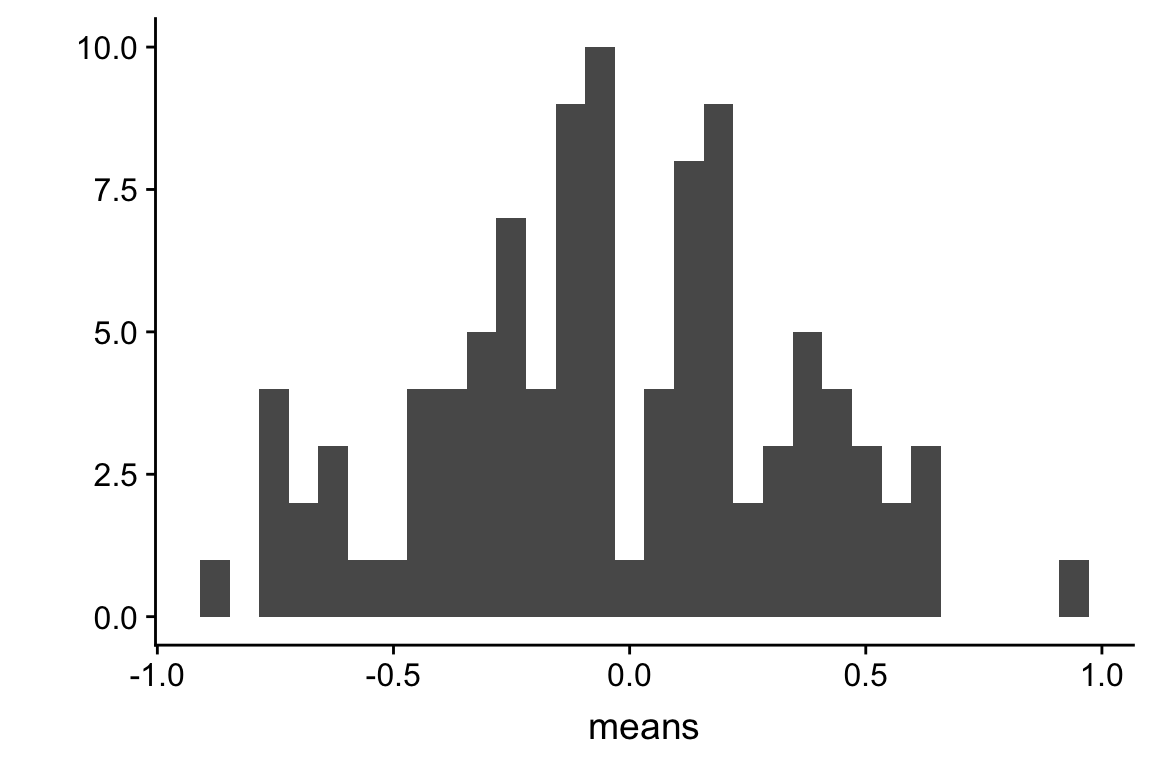
\includegraphics{Walker-elementary-statistical-modeling-draft_files/figure-latex/unnamed-chunk-6-1.pdf}

Compute the mean of the means

\begin{Shaded}
\begin{Highlighting}[]
\KeywordTok{mean}\NormalTok{(means)}
\end{Highlighting}
\end{Shaded}

\begin{verbatim}
## [1] -0.039961
\end{verbatim}

Questions

\begin{enumerate}
\def\labelenumi{\arabic{enumi}.}
\tightlist
\item
  Remember that the true mean is zero. How close, in general, are the
  sampled means to the true mean. How variable are the means? How is
  this quantified?
\item
  change n to 100, then replot. Are the means, in general, closer to the
  true mean? How variable are the means now?
\item
  Is the mean estimated with \(n=100\) closer to the truth, in general,
  then the mean estimated with \(n=6\)?
\item
  Redo with \(n=10000\)
\end{enumerate}

\subsection{part III - how do SD and SE change as sample size (n)
increases?}\label{part-iii---how-do-sd-and-se-change-as-sample-size-n-increases}

\begin{Shaded}
\begin{Highlighting}[]
\KeywordTok{mean}\NormalTok{(sds)}
\end{Highlighting}
\end{Shaded}

\begin{verbatim}
## [1] 1.017144
\end{verbatim}

Questions

\begin{enumerate}
\def\labelenumi{\arabic{enumi}.}
\tightlist
\item
  what is the mean of the standard deviations when n=6 (set p=1000)
\item
  what is the mean of the standard deviations when n=100 (set p=1000)
\item
  when n = 1000? (set p=1000)
\item
  when n = 10000? (set p=1000)
\item
  how does the mean of the standard deviations change as n increases
  (does it get smaller? or stay about the same size)
\item
  repeat the above with SEM
\end{enumerate}

\begin{Shaded}
\begin{Highlighting}[]
\KeywordTok{mean}\NormalTok{(sems)}
\end{Highlighting}
\end{Shaded}

\begin{verbatim}
## [1] 0.4152472
\end{verbatim}

Congratulations, you have just done a Monte Carlo simulation!

\subsection{\texorpdfstring{Part IV -- Generating fake data with ``for
loops''}{Part IV -- Generating fake data with for loops}}\label{part-iv-generating-fake-data-with-for-loops}

There are many other strategies for generating fake data -- two that
will be used extensively here are the funtion \texttt{rmvnorm()} and
\textbf{for loops}

\subsubsection{rmvnorm and a Covariance
Matrix}\label{rmvnorm-and-a-covariance-matrix}

We used the base R function \texttt{rnorm} above to generate
\texttt{fake\_data}, a matrix of random normal values. The columns are
generated independently of each other so the expected correlation
between any two columns is zero. The \texttt{rmvnorm()} (``random
multivariate normal'') function from the package \texttt{mvtnorm}
(``multivariate normal'') returns a matrix of random values drawn from a
multiviate normal distribution with a specified \textbf{covariance
matrix}. A covariance matrix is matrix of the variances and covariances
of the \(p\) columns of a data matrix. The \textbf{diagonal} of the
covariance matrix contains the variances of the \(p\) columns of the
data matrix and the off-diagonal elements contain the \(p(p-1)\)
pairwise covariances. The upper right set of covariances is the mirror
of the lower left set of covariates, so there are \(p(p-1)/2\) unique
covariances.

For our fake data, we want columns that are independent (E(COV) = 0) and
have expected variance of 1. This covariance matrix has a special name
-- the \textbf{identity matrix} (or sometimes ``unit'' matrix). Thus we
could use this script to generate fake data

\begin{Shaded}
\begin{Highlighting}[]
\NormalTok{n <-}\StringTok{ }\DecValTok{6} \CommentTok{# sample size}
\NormalTok{p <-}\StringTok{ }\DecValTok{10}\OperatorTok{^}\DecValTok{2} \CommentTok{# number of columns of fake data to generate}
\NormalTok{fake_data <-}\StringTok{  }\NormalTok{mvtnorm}\OperatorTok{::}\KeywordTok{rmvnorm}\NormalTok{(n, }\DataTypeTok{mean=}\KeywordTok{rep}\NormalTok{(}\DecValTok{0}\NormalTok{, p), }\DataTypeTok{sigma=}\KeywordTok{diag}\NormalTok{(p))}

\CommentTok{# compute the vectors of means, sds, and sems and the sd of the means}
\NormalTok{means <-}\StringTok{ }\KeywordTok{apply}\NormalTok{(fake_data,}\DecValTok{2}\NormalTok{,mean) }\CommentTok{# the apply function is super useful}
\NormalTok{sds <-}\StringTok{ }\KeywordTok{apply}\NormalTok{(fake_data,}\DecValTok{2}\NormalTok{,sd)}
\NormalTok{sems <-}\StringTok{ }\NormalTok{sds}\OperatorTok{/}\KeywordTok{sqrt}\NormalTok{(n)}
\KeywordTok{sd}\NormalTok{(means)}
\end{Highlighting}
\end{Shaded}

\begin{verbatim}
## [1] 0.4539342
\end{verbatim}

\begin{Shaded}
\begin{Highlighting}[]
\KeywordTok{mean}\NormalTok{(sems)}
\end{Highlighting}
\end{Shaded}

\begin{verbatim}
## [1] 0.4083748
\end{verbatim}

The vector of column means is specified using \texttt{mean=} and the
multivariate covariance matrix is specified with \texttt{sigma=} (the
lower case greek letter sigma (\(\sigma\)) is often used to denote a
population standard deviation. The upper case greek letter sigma
(\(\Sigma\)) is often used to denote a population covariance matrix).
This raises two questions

Questions.

\begin{enumerate}
\def\labelenumi{\arabic{enumi}.}
\tightlist
\item
  without using the console, what is returned with \texttt{rep(0,\ p)}?
\item
  without using the console, what is returned with \texttt{diag(p)}?
\item
  What are the \texttt{sd(means)} and \texttt{mean(sems)} comparing?
  What is the pedagogical purpose for adding this?
\end{enumerate}

Now use the console to check your answers.

\subsubsection{A for loop}\label{a-for-loop}

\begin{Shaded}
\begin{Highlighting}[]
\NormalTok{n <-}\StringTok{ }\DecValTok{6} \CommentTok{# sample size}
\NormalTok{n_iter <-}\StringTok{ }\DecValTok{10}\OperatorTok{^}\DecValTok{5} \CommentTok{# number of iterations of loop (equivalent to p)}
\NormalTok{means <-}\StringTok{ }\KeywordTok{numeric}\NormalTok{(n_iter)}
\NormalTok{sds <-}\StringTok{ }\KeywordTok{numeric}\NormalTok{(n_iter)}
\NormalTok{sems <-}\StringTok{ }\KeywordTok{numeric}\NormalTok{(n_iter)}
\ControlFlowTok{for}\NormalTok{(i }\ControlFlowTok{in} \DecValTok{1}\OperatorTok{:}\NormalTok{n_iter)\{}
\NormalTok{  y <-}\StringTok{ }\KeywordTok{rnorm}\NormalTok{(n) }\CommentTok{# mean=0 and sd=1 are default so not necessary to specify}
\NormalTok{  means[i] <-}\StringTok{ }\KeywordTok{mean}\NormalTok{(y)}
\NormalTok{  sds[i] <-}\StringTok{ }\KeywordTok{sd}\NormalTok{(y)}
\NormalTok{  sems[i] <-}\StringTok{ }\KeywordTok{sd}\NormalTok{(y)}\OperatorTok{/}\KeywordTok{sqrt}\NormalTok{(n)}
\NormalTok{\}}
\KeywordTok{sd}\NormalTok{(means)}
\end{Highlighting}
\end{Shaded}

\begin{verbatim}
## [1] 0.4090381
\end{verbatim}

\begin{Shaded}
\begin{Highlighting}[]
\KeywordTok{mean}\NormalTok{(sems)}
\end{Highlighting}
\end{Shaded}

\begin{verbatim}
## [1] 0.3883677
\end{verbatim}

Questions

\begin{enumerate}
\def\labelenumi{\arabic{enumi}.}
\tightlist
\item
  What do \texttt{sd(means)} and \texttt{mean(sems)} converge to as
  \texttt{n\_iter} is increased from 100 to 1000 to 10,000?
\item
  Do they converge to the same number?
\item
  Should they?
\item
  What is the correct number?
\end{enumerate}

Question number 4 is asking what is E(SEM), the ``expected standard
error of the mean''. There is a very easy formula to compute this. What
is it?

\chapter*{Appendix 3: Getting Started with
R}\label{appendix-3-getting-started-with-r}
\addcontentsline{toc}{chapter}{Appendix 3: Getting Started with R}

\section{Get your computer ready}\label{get-your-computer-ready}

\subsection{Install R}\label{install-r}

R is the core software

\href{https://cran.r-project.org}{Download R for your OS}

\subsection{Install R Studio}\label{install-r-studio}

R Studio is a slick (very slick) GUI interface for developing R projects

\href{https://www.rstudio.com/products/rstudio/download/}{Download R
Studio Desktop}

\subsection{Resources for installing R and R
Studio}\label{resources-for-installing-r-and-r-studio}

\href{https://medium.com/@GalarnykMichael/install-r-and-rstudio-on-windows-5f503f708027}{On
Windows}

\href{https://medium.com/@GalarnykMichael/install-r-and-rstudio-on-mac-e911606ce4f4}{On
a Mac}

\subsection{Install LaTeX}\label{install-latex}

LaTeX (``la-tek'') is necessary to use the pdf output of R Markdown.

\href{https://medium.com/@sorenlind/create-pdf-reports-using-r-r-markdown-latex-and-knitr-on-windows-10-952b0c48bfa9}{On
Windows}

\href{https://medium.com/@sorenlind/create-pdf-reports-using-r-r-markdown-latex-and-knitr-on-macos-high-sierra-e7b5705c9fd}{On
a Mac}

\section{Start learning}\label{start-learning}

\subsection{Start with Data Camp Introduction to
R}\label{start-with-data-camp-introduction-to-r}

\href{https://www.datacamp.com/courses/free-introduction-to-r}{Data
Camp: Introduction to R (free online course)}

\subsection{Then Move to Introduction to R
Studio}\label{then-move-to-introduction-to-r-studio}

\href{https://www.rstudio.com/resources/webinars/rstudio-essentials-webinar-series-part-1/}{R
Studio Essentials, Programming Part 1 (Writing code in RStudio)}

\subsection{Develop your project with an R Studio
Notebook}\label{develop-your-project-with-an-r-studio-notebook}

\href{https://www.rstudio.com/resources/webinars/getting-started-with-r-markdown/}{Getting
Started with R Markdown}

\href{https://www.rstudio.com/resources/webinars/introducing-notebooks-with-r-markdown/}{Introducing
Notebooks with R Markdown}

\section{Getting Data into R}\label{getting-data-into-r}

\href{https://www.rstudio.com/resources/webinars/getting-your-data-into-r/}{Getting
your data into R}

\section{Additional R learning
resources}\label{additional-r-learning-resources}

\href{https://bookdown.org/chesterismay/rbasics/}{Getting used to R,
RStudio, and R Markdown}

\href{https://www.rstudio.com/resources/webinars/}{Link to list of R
Studio webinars}

\href{https://www.rstudio.com/resources/cheatsheets/}{Link to set of R
package cheat sheets (amazing!)}

\href{https://bookdown.org}{Bookdown online books}

\section{Packages used extensively in this
text}\label{packages-used-extensively-in-this-text}

\begin{enumerate}
\def\labelenumi{\arabic{enumi}.}
\tightlist
\item
  ggplot2
\item
  data.table
\item
  mvtnorm
\item
  lme4
\item
  nlme
\item
  emmeans
\item
  readxl
\item
  reshape2
\end{enumerate}

\href{http://r4ds.had.co.nz/data-visualisation.html}{Data Visualisation
chapter from \emph{R for Data Science}}

\href{http://r4ds.had.co.nz/graphics-for-communication.html}{Graphics
for communication chapter from \emph{R for Data Science}}

Youtube: \href{https://www.youtube.com/watch?v=pc1ARG6kbAM}{An
Introduction to The data.table Package}

Coursera:
\href{https://www.coursera.org/learn/data-cleaning/lecture/trMZ7/the-data-table-package}{The
data.table Package}

\chapter*{Appendix 4: Online Resources for Getting Started with Linear
Modeling in
R}\label{appendix-4-online-resources-for-getting-started-with-linear-modeling-in-r}
\addcontentsline{toc}{chapter}{Appendix 4: Online Resources for Getting
Started with Linear Modeling in R}

\href{https://leanpub.com/regmods}{Regression Models for Data Science in
R by Brian Caffo}

\href{https://bookdown.org/roback/bookdown-bysh/}{Broadening Your
Statistical Horizons: Generalized Linear Models and Multilevel Models by
J. Legler and P. Roback}

\href{https://bookdown.org/rdpeng/artofdatascience/}{The Art of Data
Science by Roger D. Peng and Elizabeth Matsui}

\bibliography{book.bib,packages.bib}


\end{document}
